\section{Circuitos pasaaltos, pasabanda y rechazabanda}
En esta secci\'on se analizaran 3 circuitos en los cuales se dispone una configuraci\'on alternativa a la propuesta
en la secci\'on donde se analiz\'o el circuito pasabajos. Para cada uno de estos circuitos se estudiar\'a o caracterizar\'a
sus funci\'on transferencia, respuesta en frecuencia y respuesta al escal\'on.

\subsection{Circuito Pasabanda}

\begin{figure}[H]
    \centering
    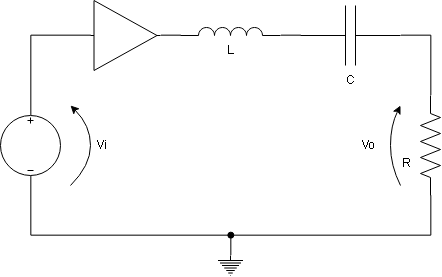
\includegraphics[scale=0.5]{Recursos/circuito_pasabanda.png}
    \caption{Circuito pasabanda}
    \label{fig:circuito_pasabanda}
\end{figure}

\subsubsection{An\'alisis te\'orico}
Para caracterizar el sistema dado por el circuito propuesto, considerando el sistema lti, causal y bibo-estable,
luego se plantea un divisor de tensi\'on en la salida para obtener la relaci\'on de tensi\'on y con ello encontrar la funci\'on
transferencia.

\begin{align*}
    & H(s) = \frac{s \cdot C \cdot R}{1 + s \cdot C \cdot R + s^{2} \cdot L \cdot C} \Rightarrow \\
    & \Delta \omega = C \cdot R \cdot \omega_o^{2} \\
    & \omega_o = \frac{1}{ \sqrt{L \cdot C} }
\end{align*}

\begin{equation}
    H(s) = \frac{\frac{s \cdot \Delta \omega}{\omega_o^{2}}}{1 + \frac{s \cdot \Delta \omega}{\omega_o^{2}} + \left( \frac{s}{\omega_o} \right)^{2}}
\end{equation}

Si bien la notaci\'on empleada es v\'alida para todos los sistemas de segundo orden, se decide emplear esta porque por su forma,
la funci\'on transferencia ya da una noci\'on de un filtro pasabando, con lo cual dejar visible alguno de los par\'ametros que permiten
definir al pasabanda como lo es el ancho de banda y la frecuencia de corte, se lo consider\'o un buen criterio. Entonces, buscando que el sistema
se encuentre con un valor de $\xi = 0.4$, es necesario que luego al igual que antes la resistencia valga idealmente $R \approx 120.6 \Omega$ con
lo cual tiene una $\omega_o = 2 \pi \cdot 47,987kHz$ y un $\Delta \omega = 2\pi \cdot 38.38kHz$.

\begin{figure}[H]
    \centering
    \begin{tabular}{c c}
        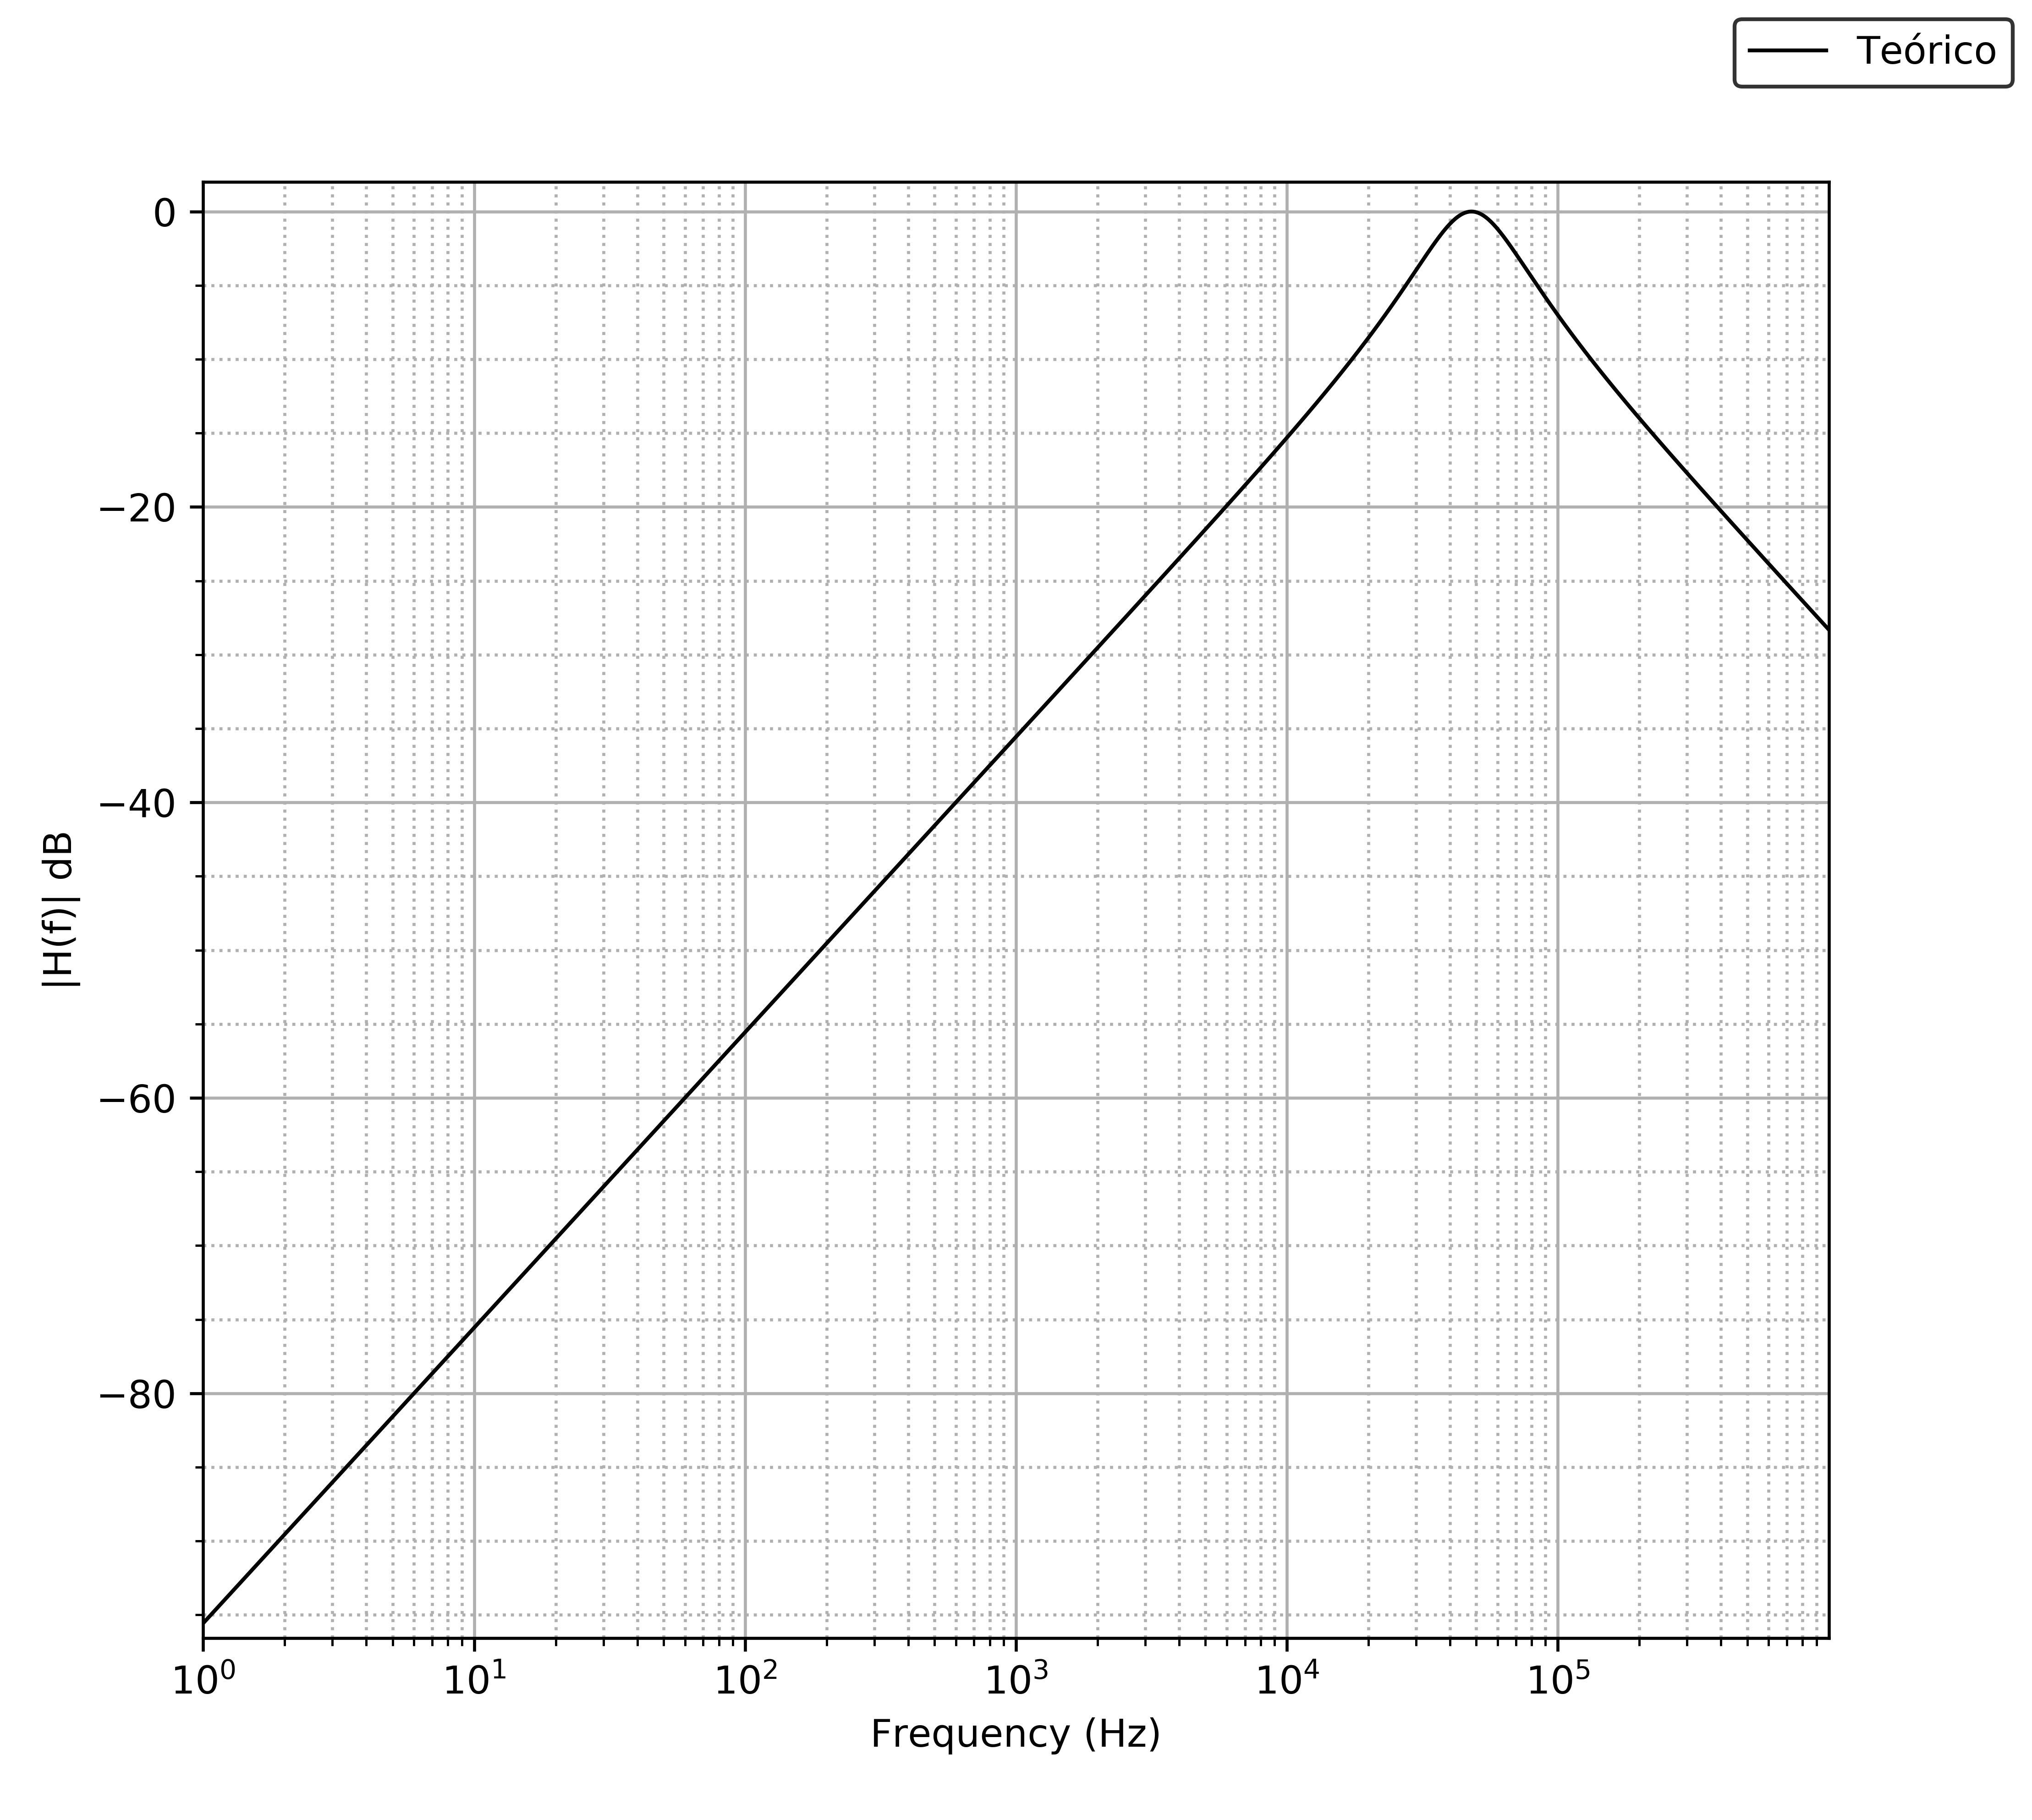
\includegraphics[scale=0.4]{Recursos/bode_teorico_pasabanda_modulo.png}
        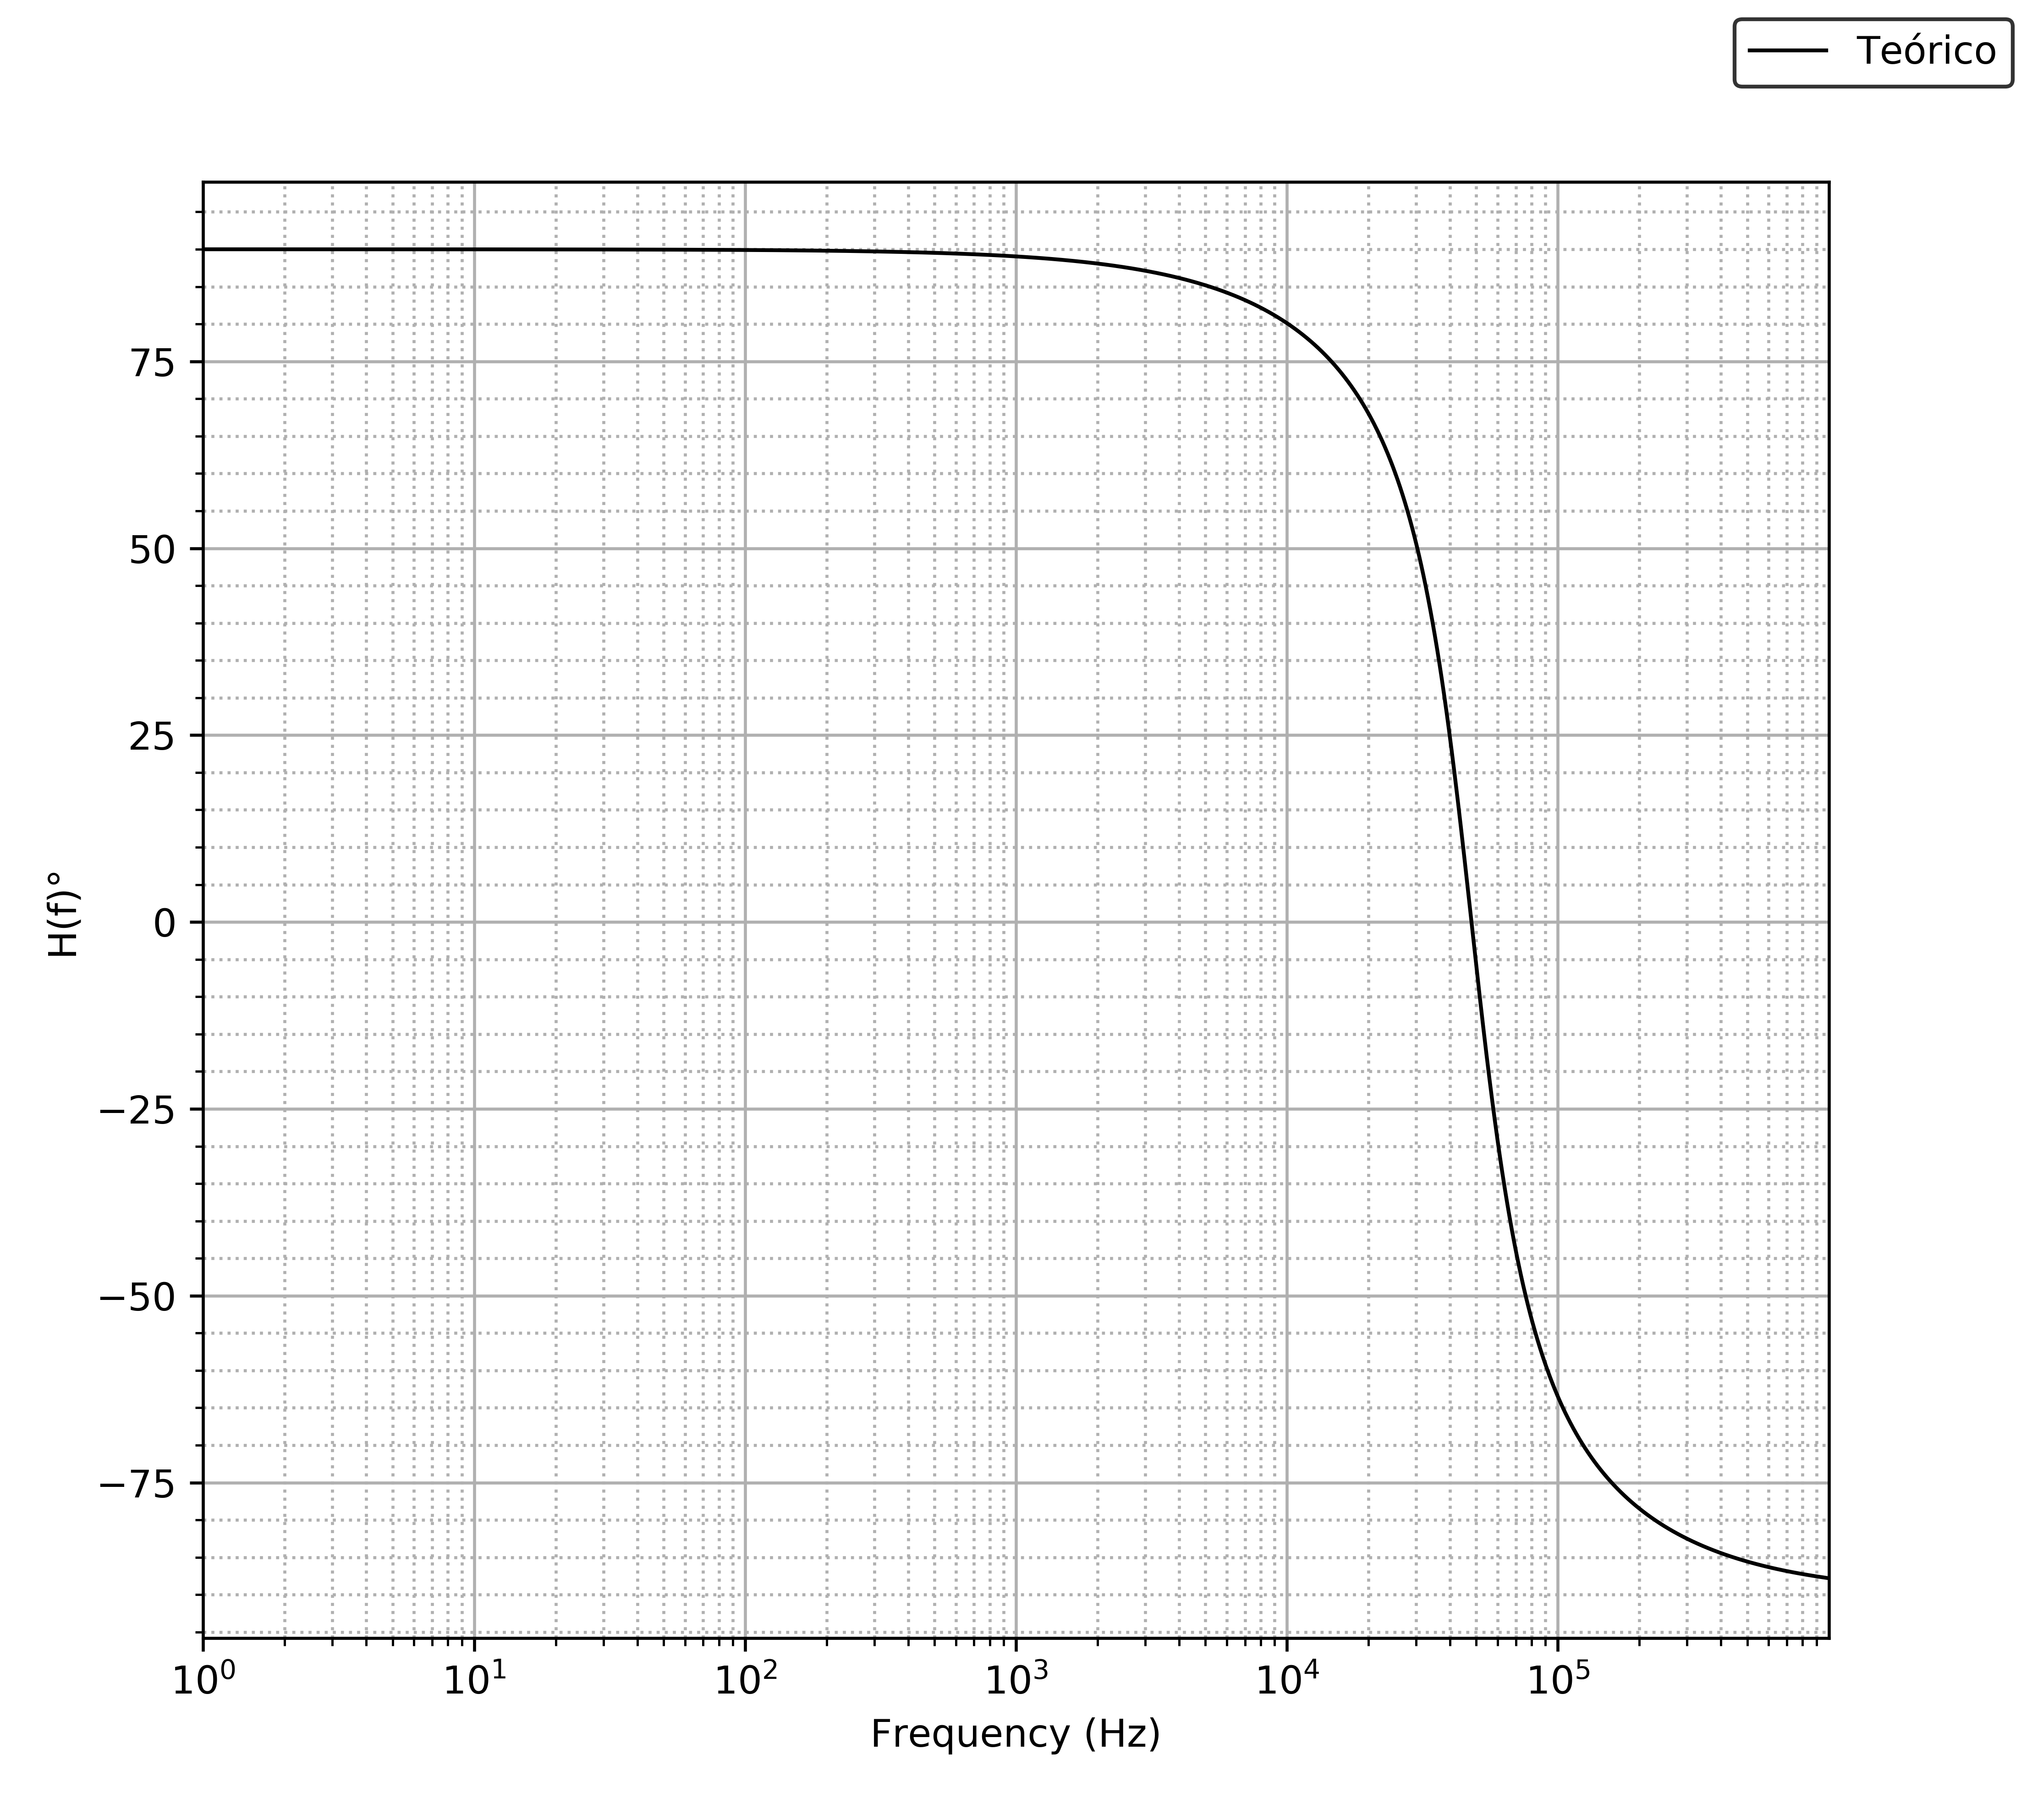
\includegraphics[scale=0.4]{Recursos/bode_teorico_pasabanda_fase.png}
    \end{tabular}
    \caption{Diagramas de bode te\'orico del circuito pasabanda}
    \label{fig:bode_pasabanda_teorico}
\end{figure}

Por otro lado, analizando el comportamiento del circuito desde un punto de vista temporal, si se aplica en la entrada una se\~nal cuadrada que simule un escal\'on
con una amplitud arbitraria de valor A definida por limitaciones f\'isicas de la pr\'actica, luego se obtiene $V_o(s) = V_i(s) \cdot H(s)$ y se antitransforma por Laplace
para obtener la respuesta temporal al escal\'on que caracteriza a este sistema. Vale mencionar, que se reacomoda la expresi\'on de la funci\'on transferencia para facilitar el trabajo
matem\'atica, y se reutilizan las definiciones de los par\'ametros del circuito pasabajos.

\begin{equation*}
    V_o(s) = V_i(s) \cdot H(s) = \frac{A}{s} \cdot \frac{2 \cdot \alpha \cdot A}{(s + \alpha)^{2} + \omega_d^{2}}
    \Rightarrow v_o(t) = \frac{2 \cdot A \cdot \xi}{\sqrt{1 - \xi^{2}}} \cdot e^{- \alpha \cdot t} \cdot \sin{(\omega_d \cdot t)}
\end{equation*}

Si en esta \'ultima expresi\'on se deriva en b\'usqueda del punto m\'aximo para encontrar el sobrepico, y luego se eval\'ua para hallar su magnitud,
realizando los siguientes pasos se llega a que:

\begin{align*}
    \frac{\delta v_o(t_p)}{\delta t} = 0 \Leftrightarrow t_p = \frac{\arctan{(\frac{\sqrt{1 - \xi^{2}}}{\xi})}}{\omega_d} \\
    \Rightarrow
    vo_{max} = A \cdot \xi \cdot e^{\frac{- \xi}{\sqrt{1 - \xi^{2}}} \cdot \arctan{(\frac{\sqrt{1 - \xi^{2}}}{\xi})}} \\
    \Rightarrow 
    M_p = \xi \cdot e^{\frac{- \xi}{\sqrt{1 - \xi^{2}}} \cdot \arctan{(\frac{\sqrt{1 - \xi^{2}}}{\xi})}}
\end{align*}

Luego si se repite el criterio de que el tiempo de establecimiento se da cuando la oscilaci\'on amortiguada tiene por envolvente
un $5 \%$ de lo que le corresponde a la amplitud del escal\'on de entrada. Entonces se obtiene que el transitorio deber'ia durar aproximadamente:

\begin{equation}
    t_s = \frac{ \ln{(\frac{0.05 \cdot \sqrt{1 - \xi^{2}}}{2 \cdot \xi})} }{- \xi \cdot \omega_o}
\end{equation}

Finalmente, si se eval\'uan estas expresiones para caracterizar la respuesta al escal\'on a nivel te\'orico, se obtiene:

\begin{table}[H]
    \centering
    \begin{tabular}{c c c c c c c}
        $t_s$ & $t_p$ & $M_p$ & $Q$ & $f_o$ & $\Delta f$ & $Sistema$ \\
        \hline \\
        $18.97 \mu s$ & $4.195 \mu s$ & $0.2412$ & $1.25$ & $47,986kHz$ & $38,38kHz$ & $Subamortiguado$ \\
        \hline
    \end{tabular}
\end{table}

\subsubsection{Resultados}
Para el circuito pasabanda se utilizaron los mismos componentes que en el punto 2. Adem\'as se utiliz\'o un potenciometro para calibrar la resistencia tal que se alcance el $\xi = 0.4$. 


A continuaci\'on se presentan los resultados de las mediciones de la respuesta natural del circuito, as\'i como una captura de pantala con la resistencia ya calibrada:


\begin{table}[H]
    \centering
    \begin{tabular}{c c c c c}
        $t_s$ & $t_p$ & $M_p$ & $f_o$ & $Sistema$ \\
        \hline \\
        $19.07 \mu s$ & $5.05 \mu s$ & $0.24$ & $48,544kHz$ & $Subamortiguado$ \\
        \hline
    \end{tabular}
    \label{tab:natural_pasabanda}
\end{table}

\begin{figure}[H]
	\centering
	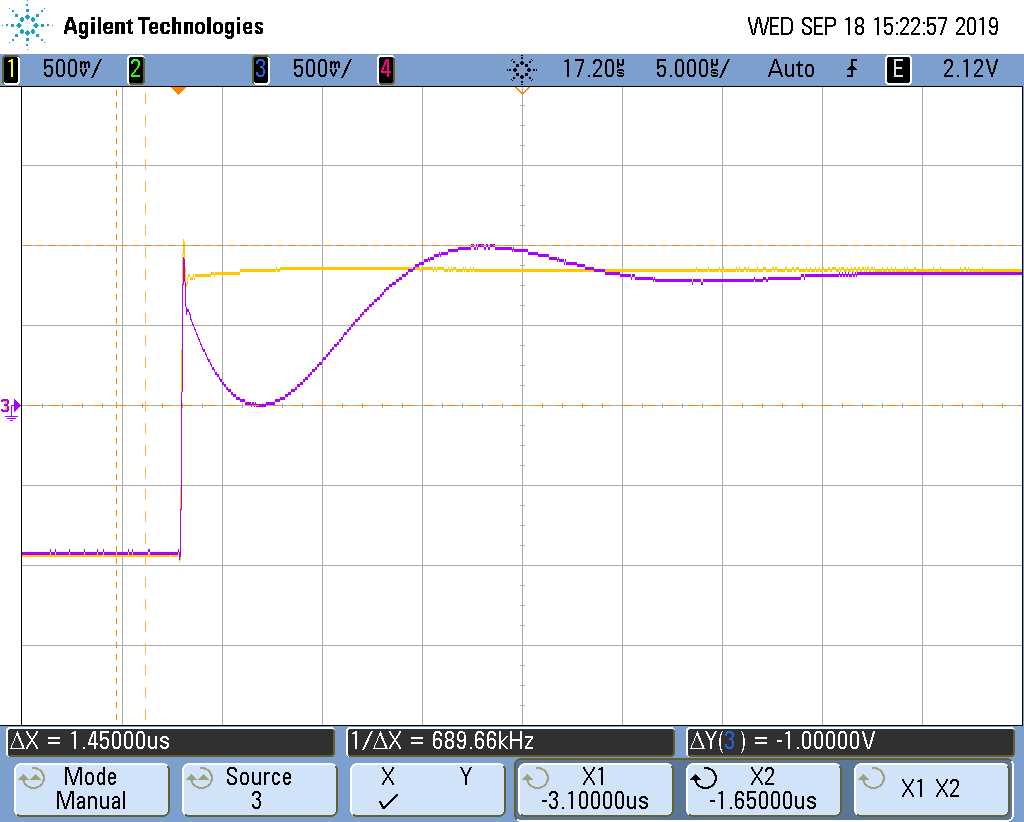
\includegraphics[scale=0.3]{../Mediciones/Osciloscopio/Rechazabanda_respuesta_escalon/scope_5.png}
\end{figure}

Los resultados de la tabla \ref{tab:natural_pasabanda} se corresponden en gran medida con los datos te\'oricos esperados presentados en la secci\'on anterior. Cabe mencionar que la resistencia con la cual se lleg\'o a dichos resultados no fue la esperada, sino que tuvo un valor de   94,4 ohm. Lo anterior pudo deverse a la resistencia de salida del buffer utilizado sumada a las resistencia propias de los componentes no ideales presentes en el circuito. 


Por \'ultimo se presenta el an\'alisis en frecuencia del ciruito, los diagramas de Bode medidos y su posterior interpretaci\'on:

\begin{figure}[H]
    \centering
    \begin{tabular}{c c}
        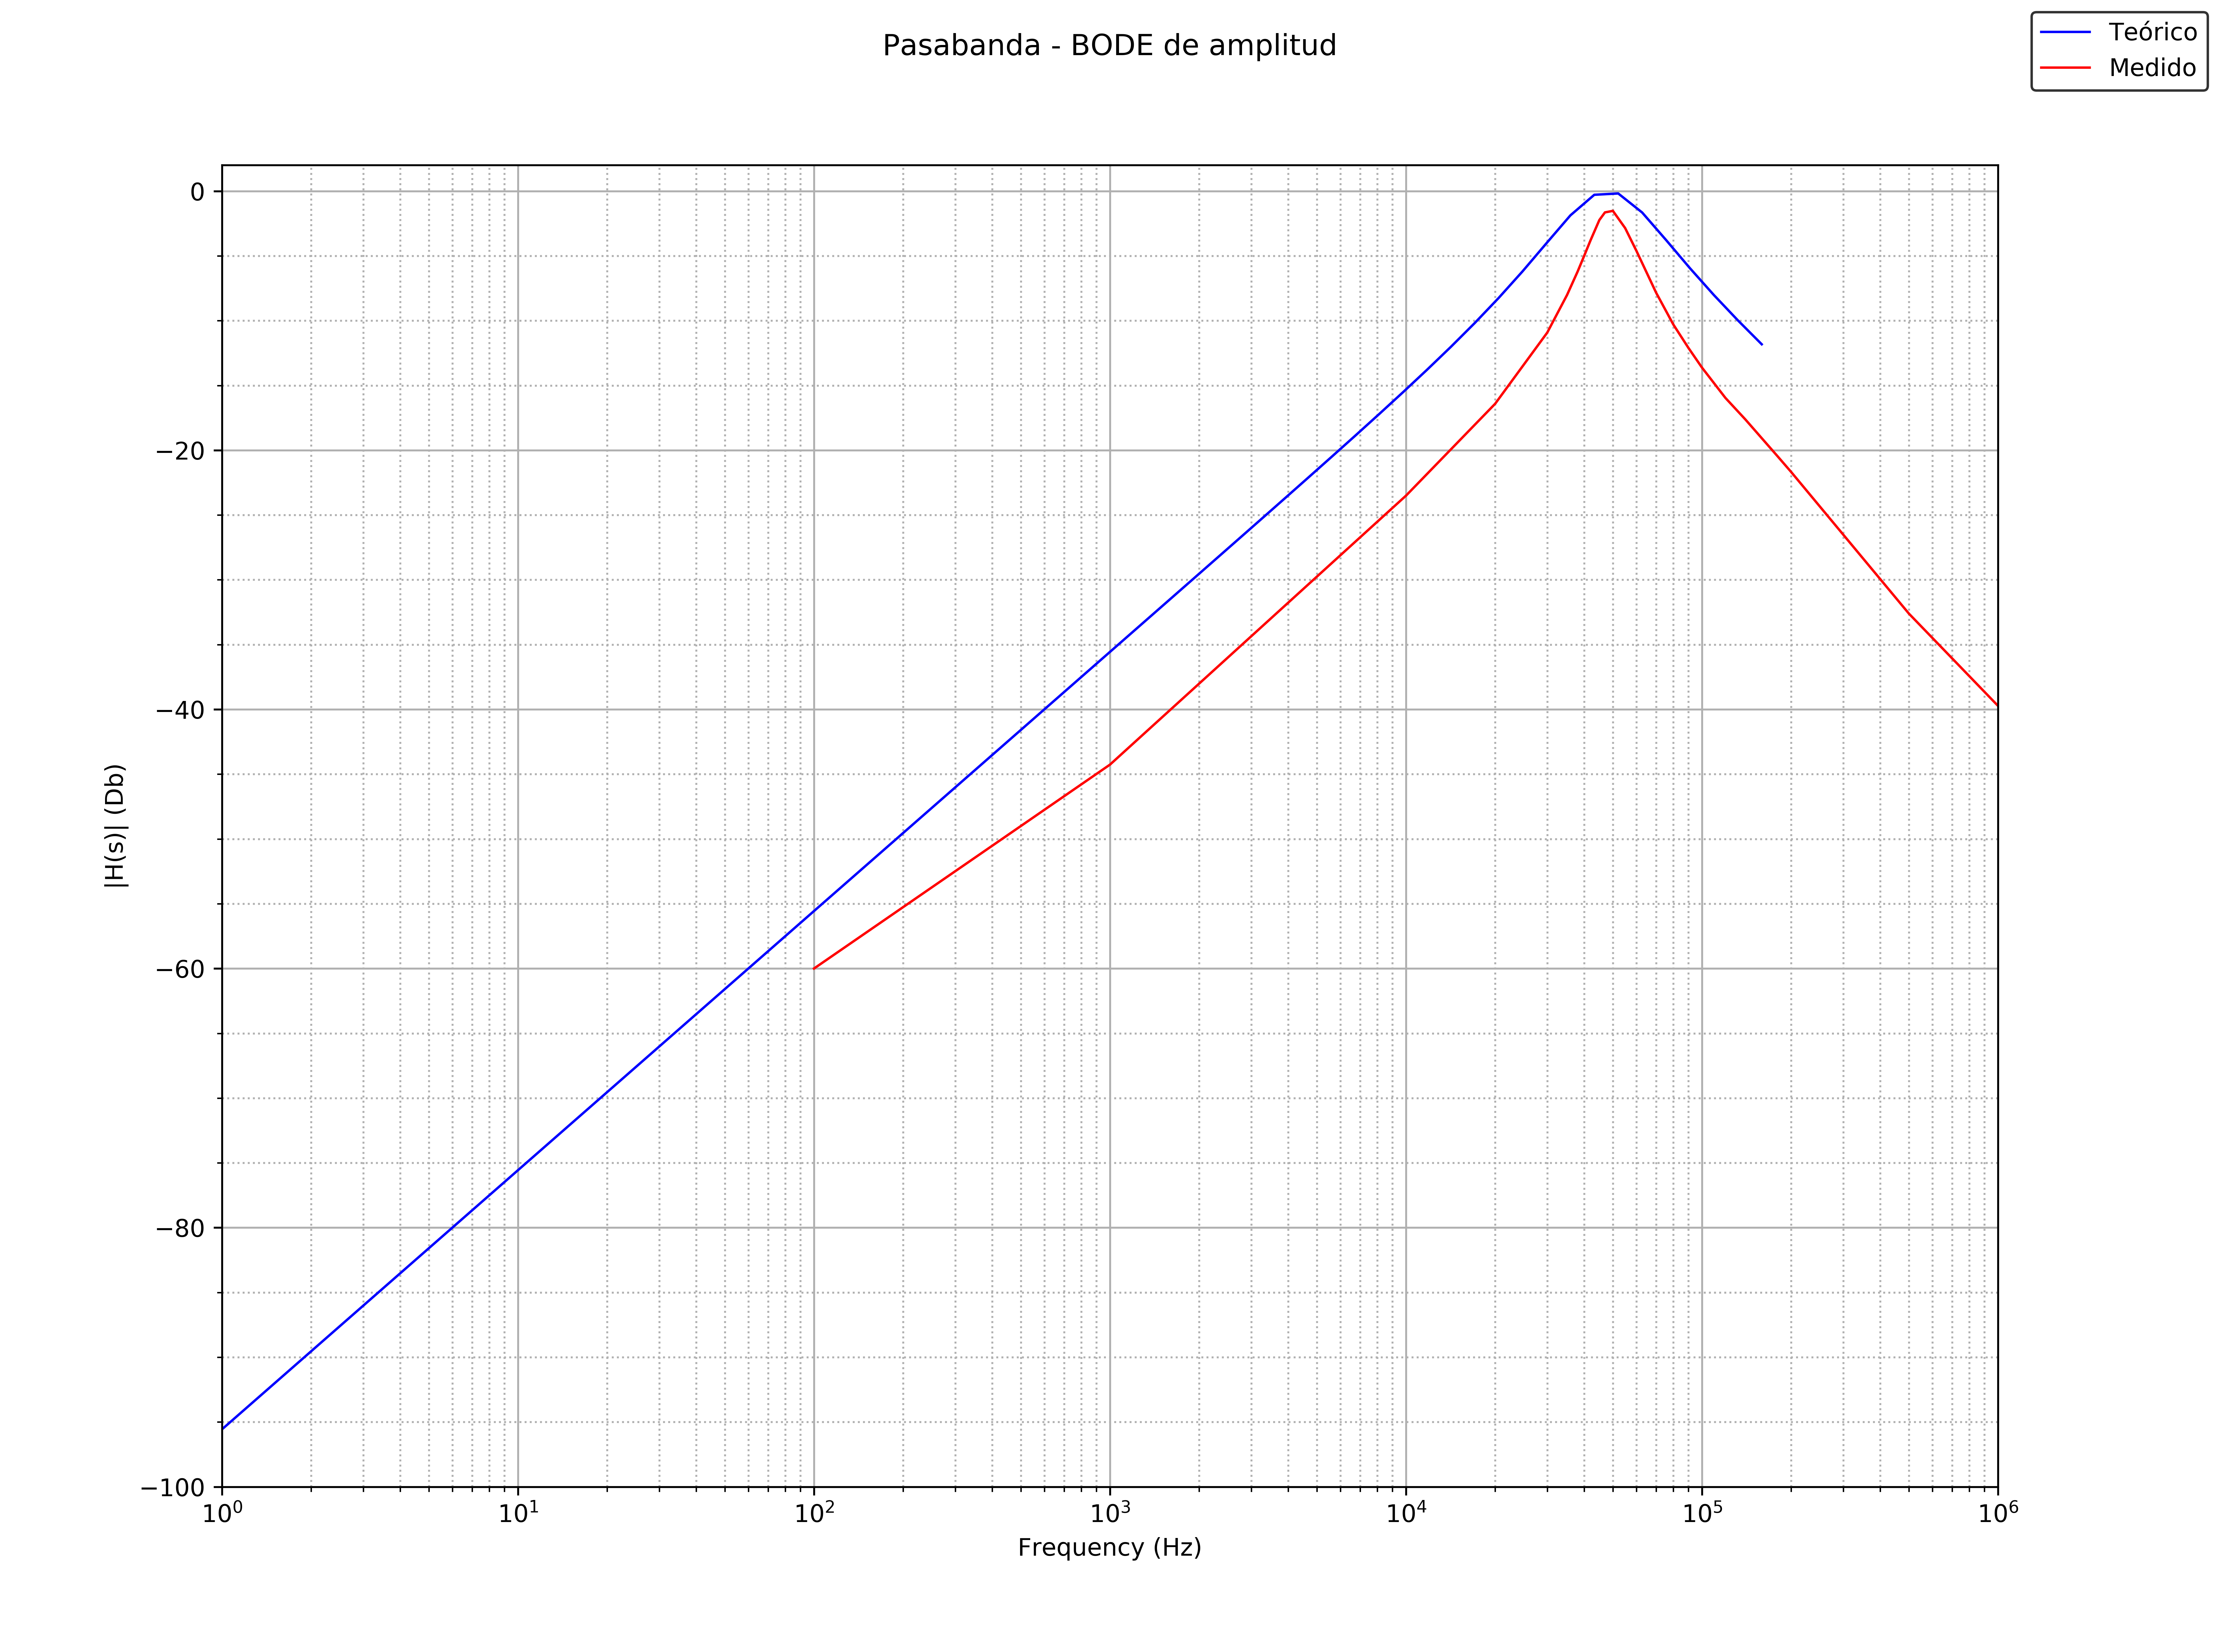
\includegraphics[scale=0.3]{Recursos/ej4/pasabanda_amplitud.png}
        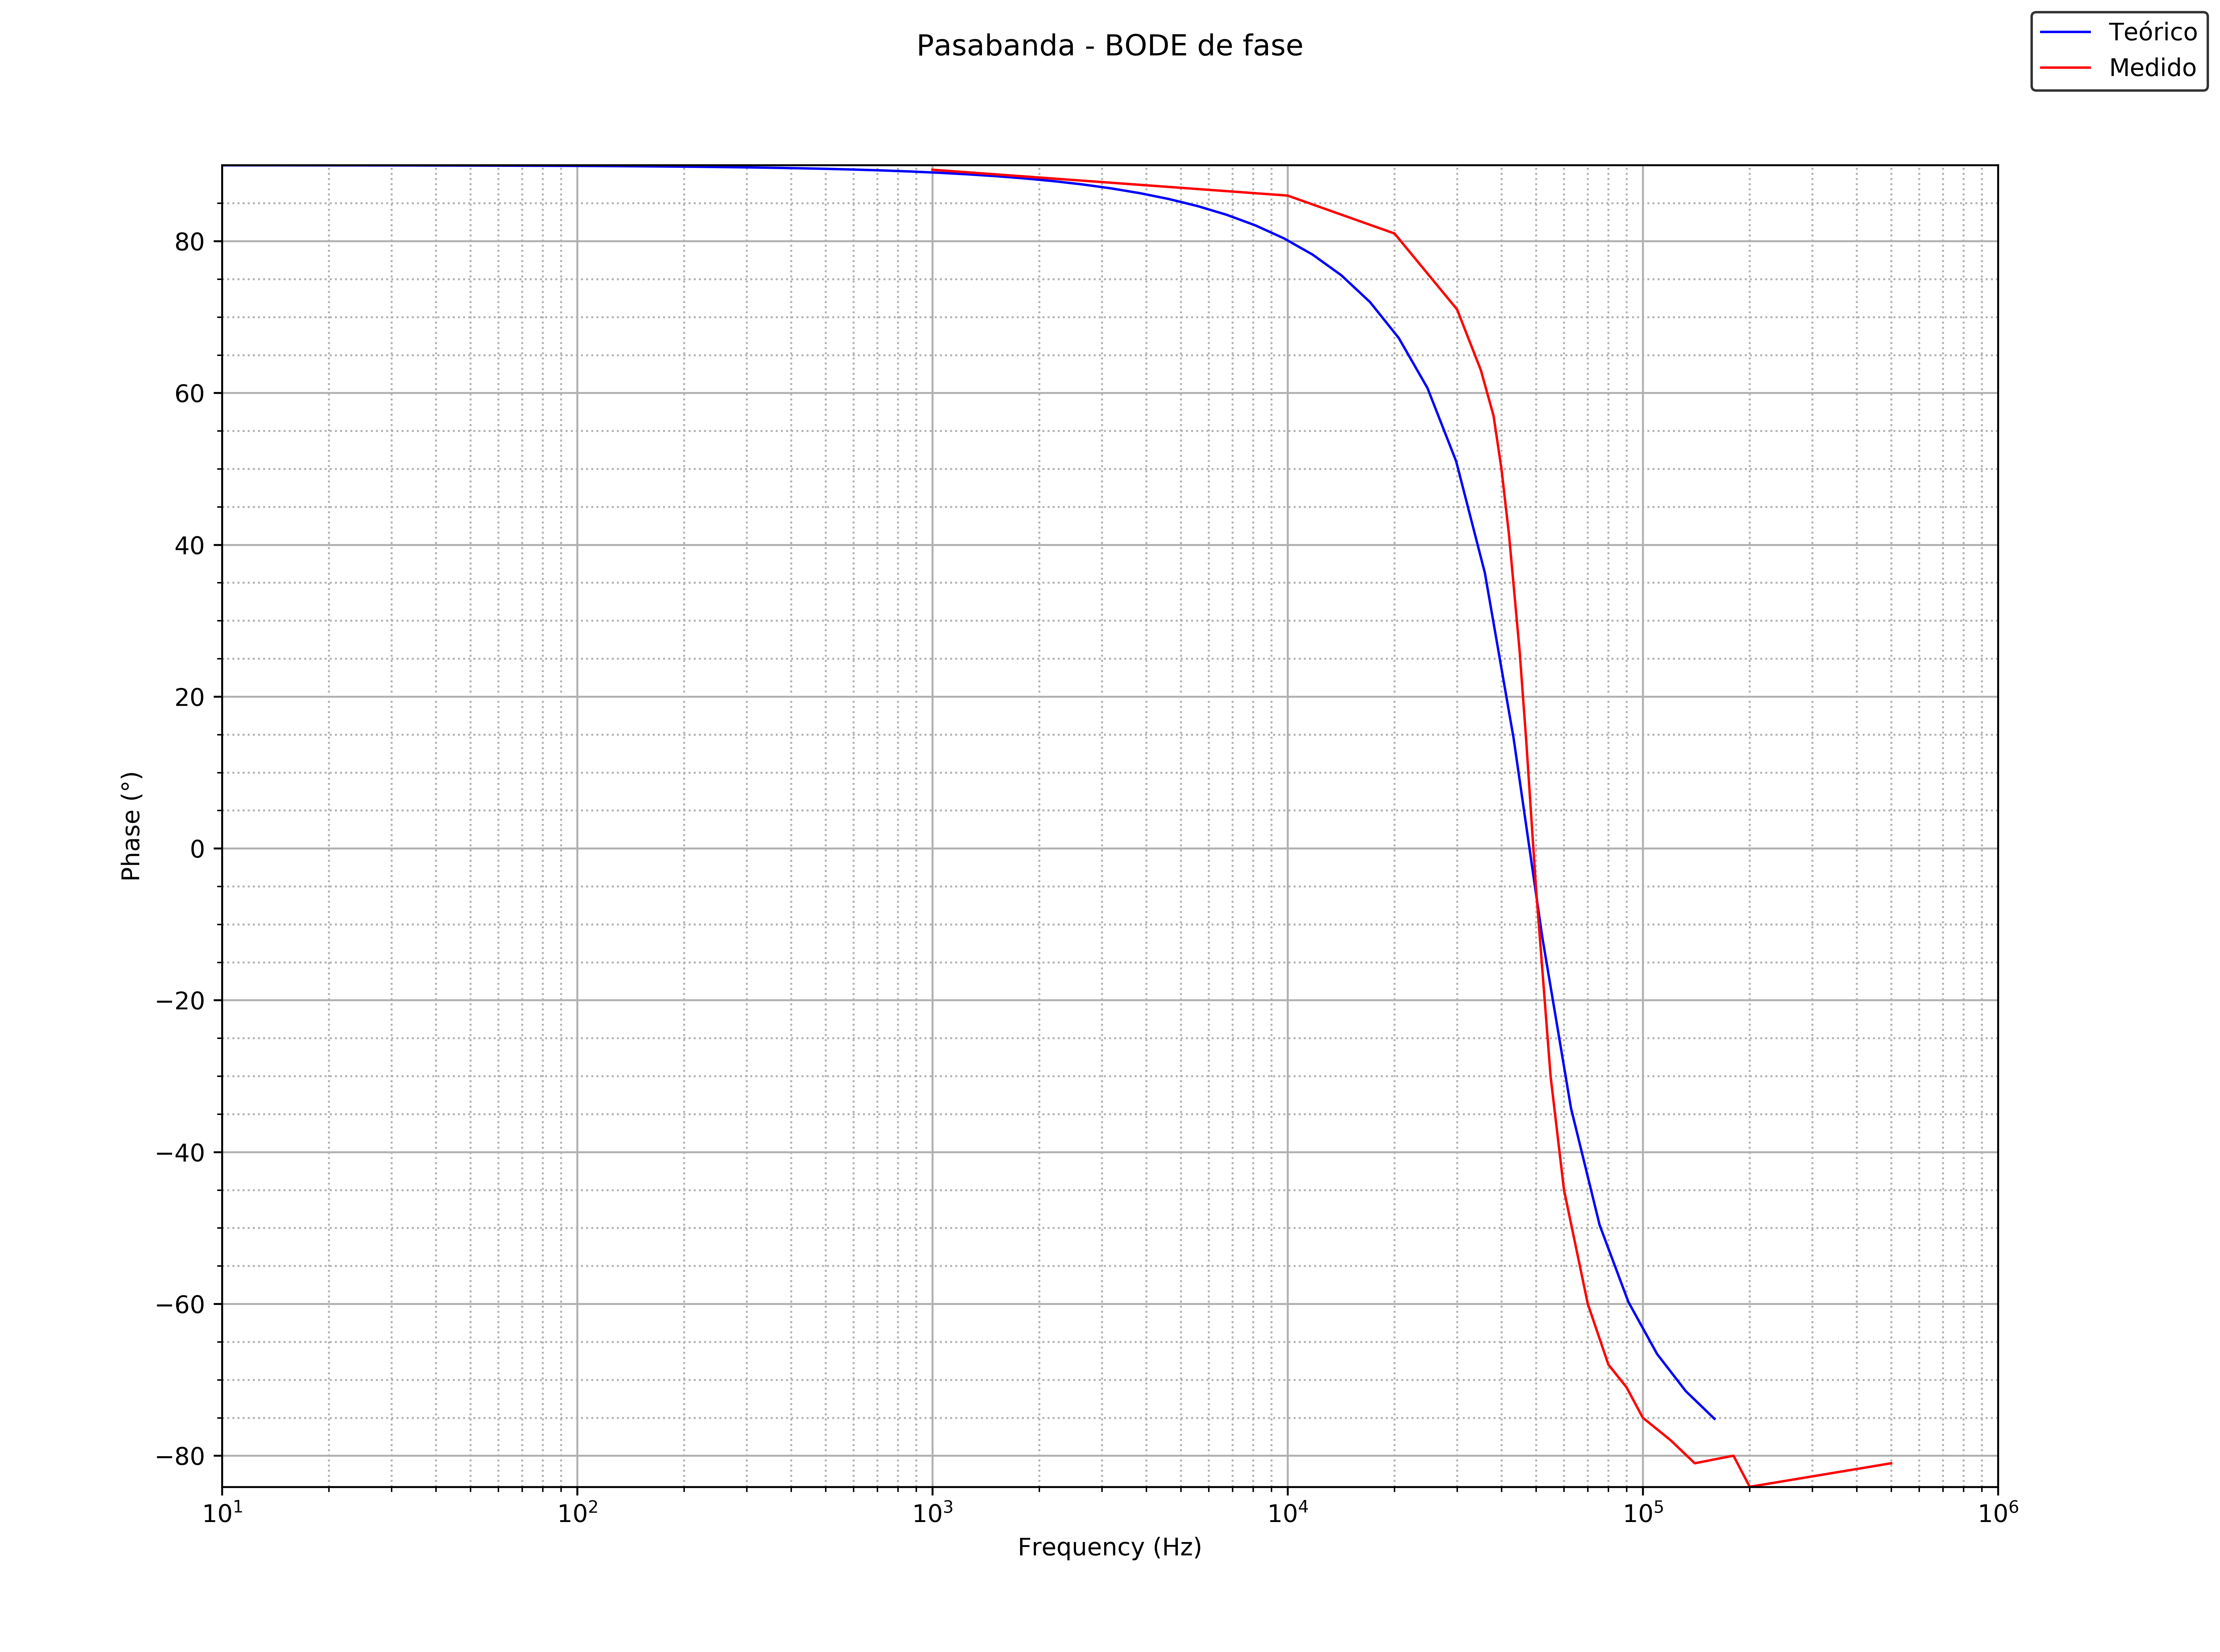
\includegraphics[scale=0.3]{Recursos/ej4/pasabanda_fase.png}
    \end{tabular}
    \caption{Diagramas de bode teóricos y simulados circuito pasabanda}
    \label{fig:bode_pasabanda}
\end{figure}

Del primer gráfico puede observarse que a pesar de no haberse llegado a la ganancia ideal del pasabanda, las pendientes antes y despues de la banda pasante son correctas. Dado que un filtro pasa banda ideal transmite, sin distorsion, todas las señales contenidas en en una banda de frecuencias y atenúa completamente las frecuencias afuera de dicha banda, los resultaods obtenidos son satisfactorios. Más aún, si se considera que tanto el capacitor como la bobina utilizados no se comportan como tales llegadas frecuencias lo suficientemente altas, y que aparecen resistencias adicionales al agregar los modelos equivalentes de los mismos. Conclusiones similares pueden sacarse respecto al gráfico en fase del circuito, el cual no tiene un cambio de fase tan abrupto como el modelo teórico, pero si el comportamiento general esperado de tal filtro. Para las últiams mediciones en el caso de la fase ocurre algo similar que en el gráfico de amplitud, a altas frecuecnias tanto la bobina como el capacitor exiben un comportamiento distinto al ideal, el cual distorsiona los resultaods empíricos. 



\subsection{Circuito Pasaaltos}

\begin{figure}[H]
    \centering
    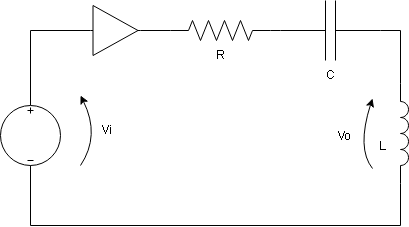
\includegraphics[scale=0.5]{Recursos/circuito_pasaaltos.png}
    \caption{Circuito pasaaltos}
    \label{fig:circuito_pasaaltos}
\end{figure}

\subsubsection{An\'alisis te\'orico}
Bajos las mismas suposiciones sobre el sistema que se vienen realizando para los circuitos anteriores,
se busca la funci\'on transferencia realizando el divisor de tensi\'on y se obtiene la siguiente transferencia. Vale mencionar,
que para no sobrecargar la notaci\'on de la funci\'on transferencia, se reutilizan par\'ametros ya definidos anteriormente
para un sistema de segundo orden.

\begin{equation}
    H(s) = \frac{\left(\frac{s}{\omega_o} \right)^{2}}{1 + s \cdot \frac{2 \cdot \xi}{\omega_o} + \left( \frac{s}{\omega_o} \right)^{2}}
    \label{eq:trans_PA}
\end{equation}

Obteniendo num\'ericamente los valores que se reemplazan en esta funci\'on transferencia, se obtiene el diagrama de bode te\'orico que permite establecer
que el comportamiento de este circuito es el de un filtro pasaaltos, puesto que no aten\'ua para frecuencias muy altas, como si lo hace para frecuencias bajas o 
inferiores a la frecuencia de corte del sistema.

\begin{figure}[H]
    \centering
    \begin{tabular}{c c}
        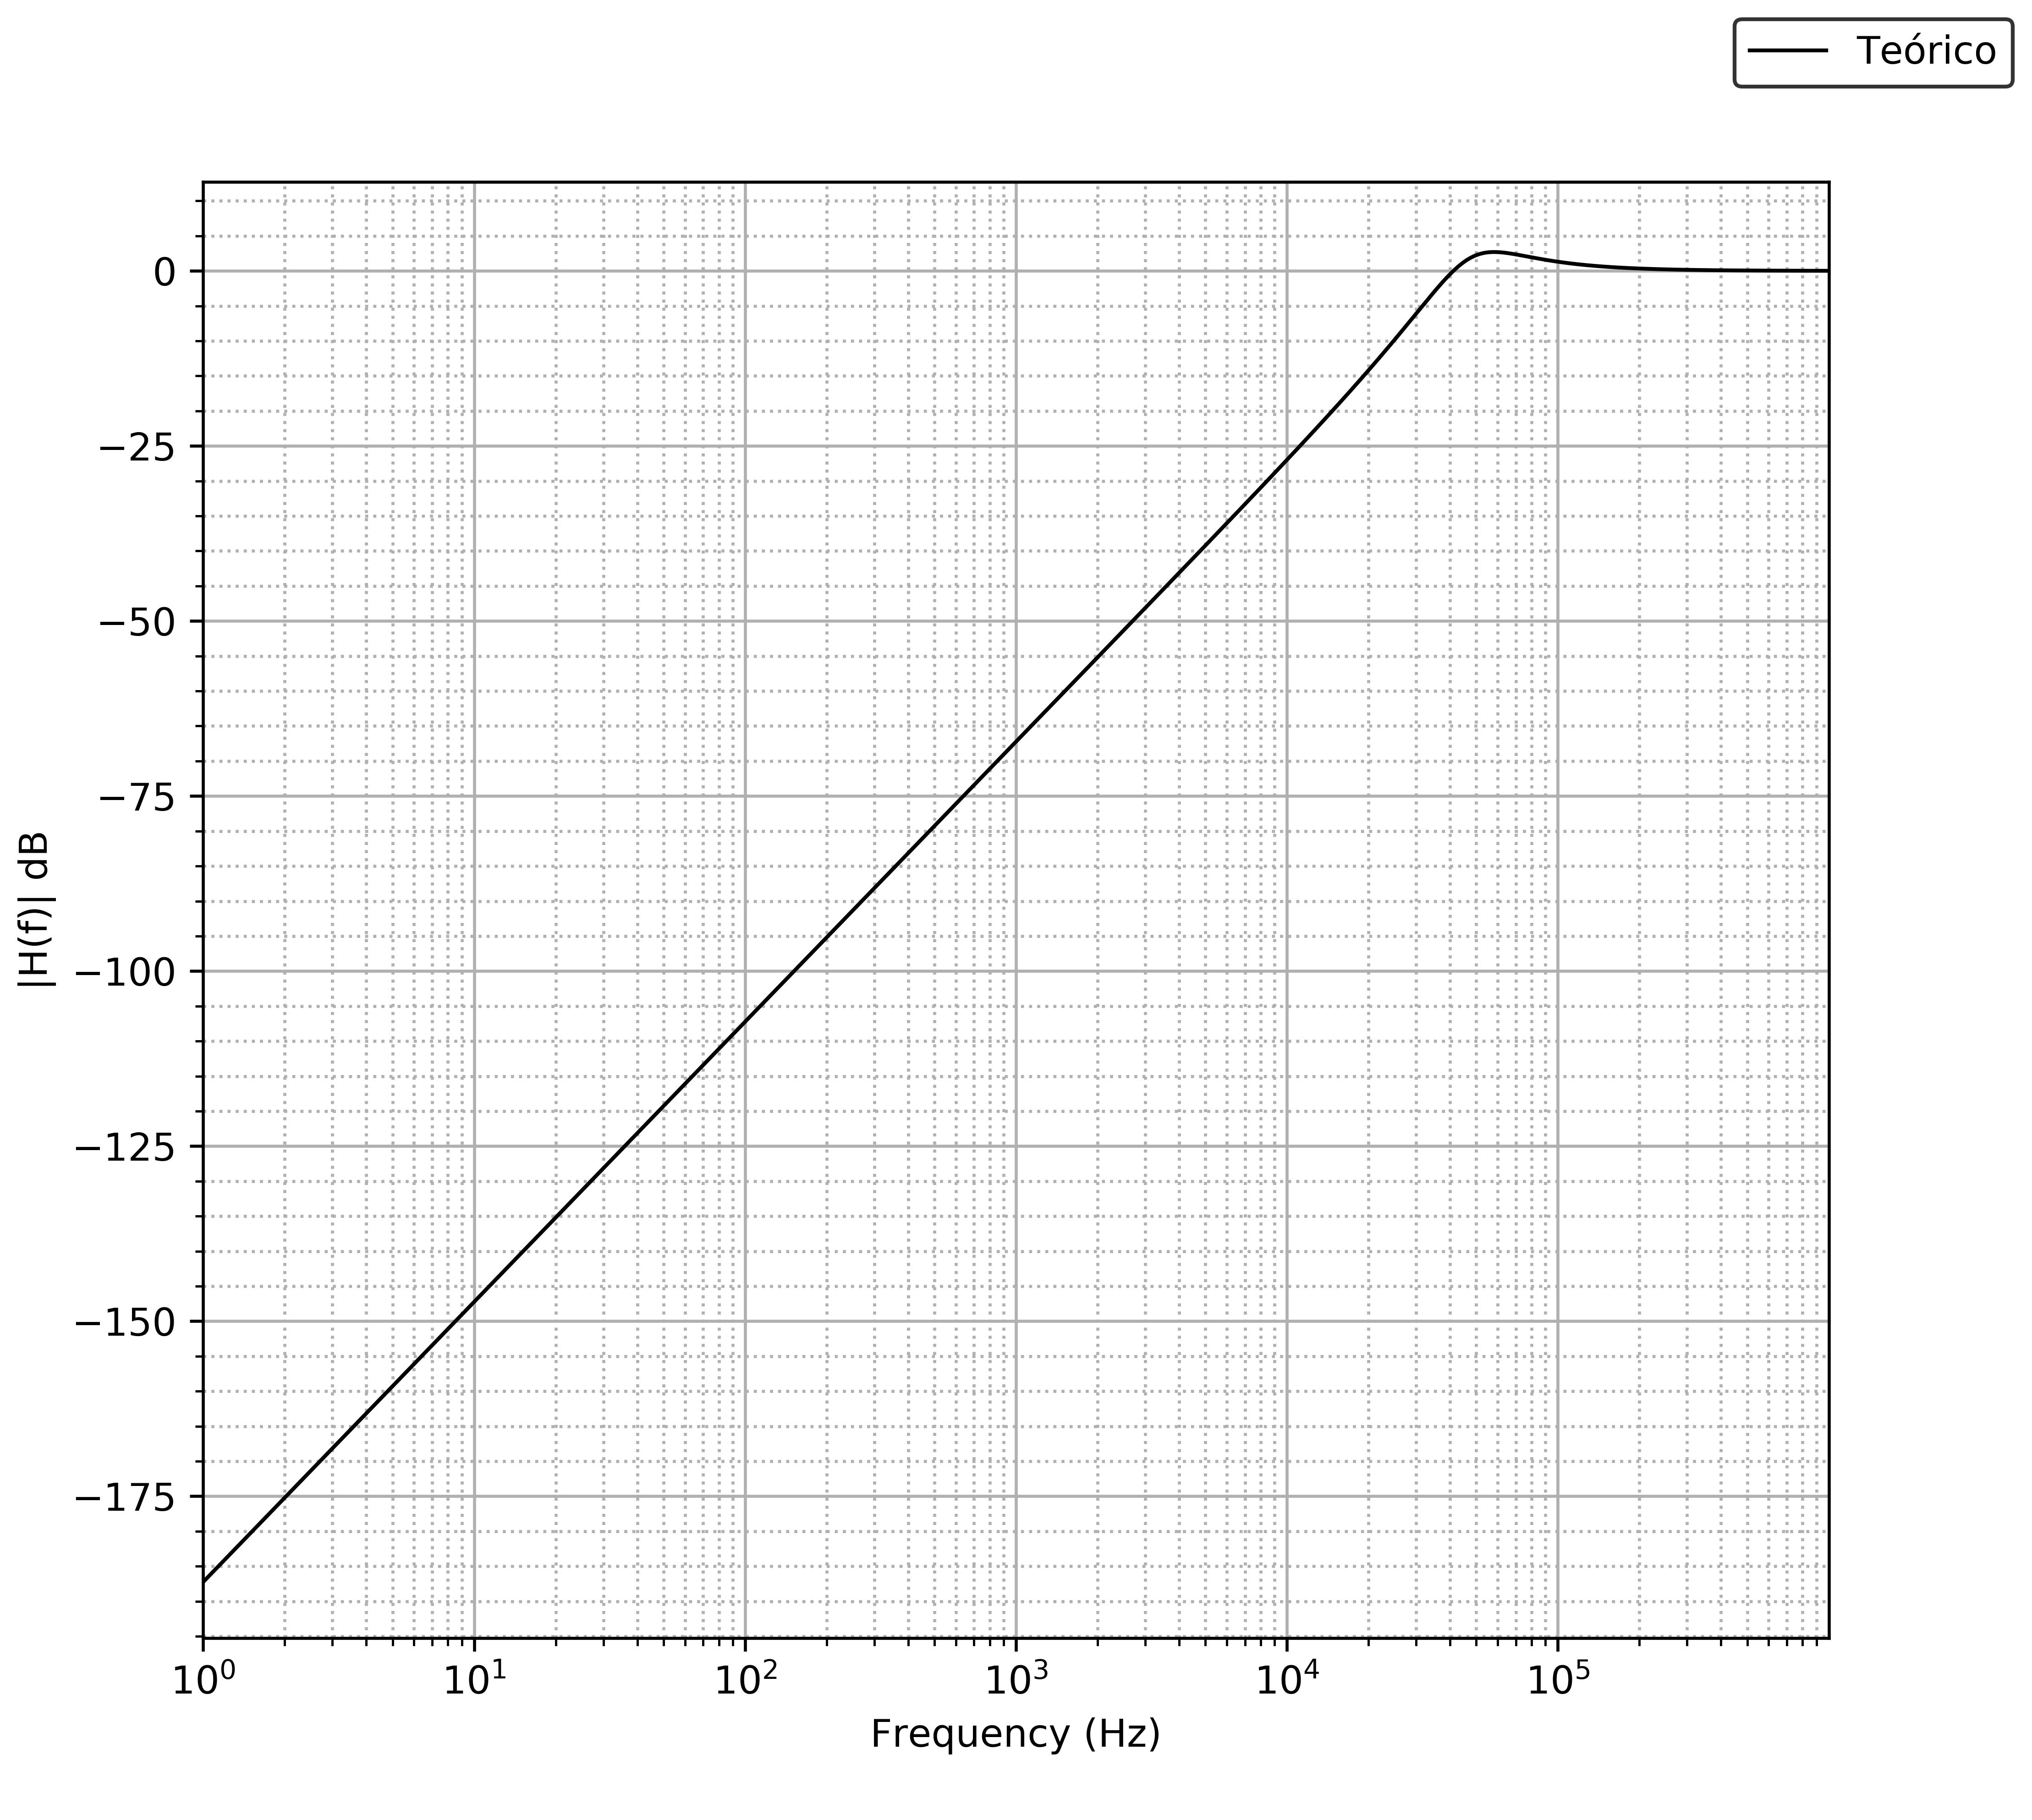
\includegraphics[scale=0.3]{Recursos/bode_teorico_pasaaltos_modulo.png}
        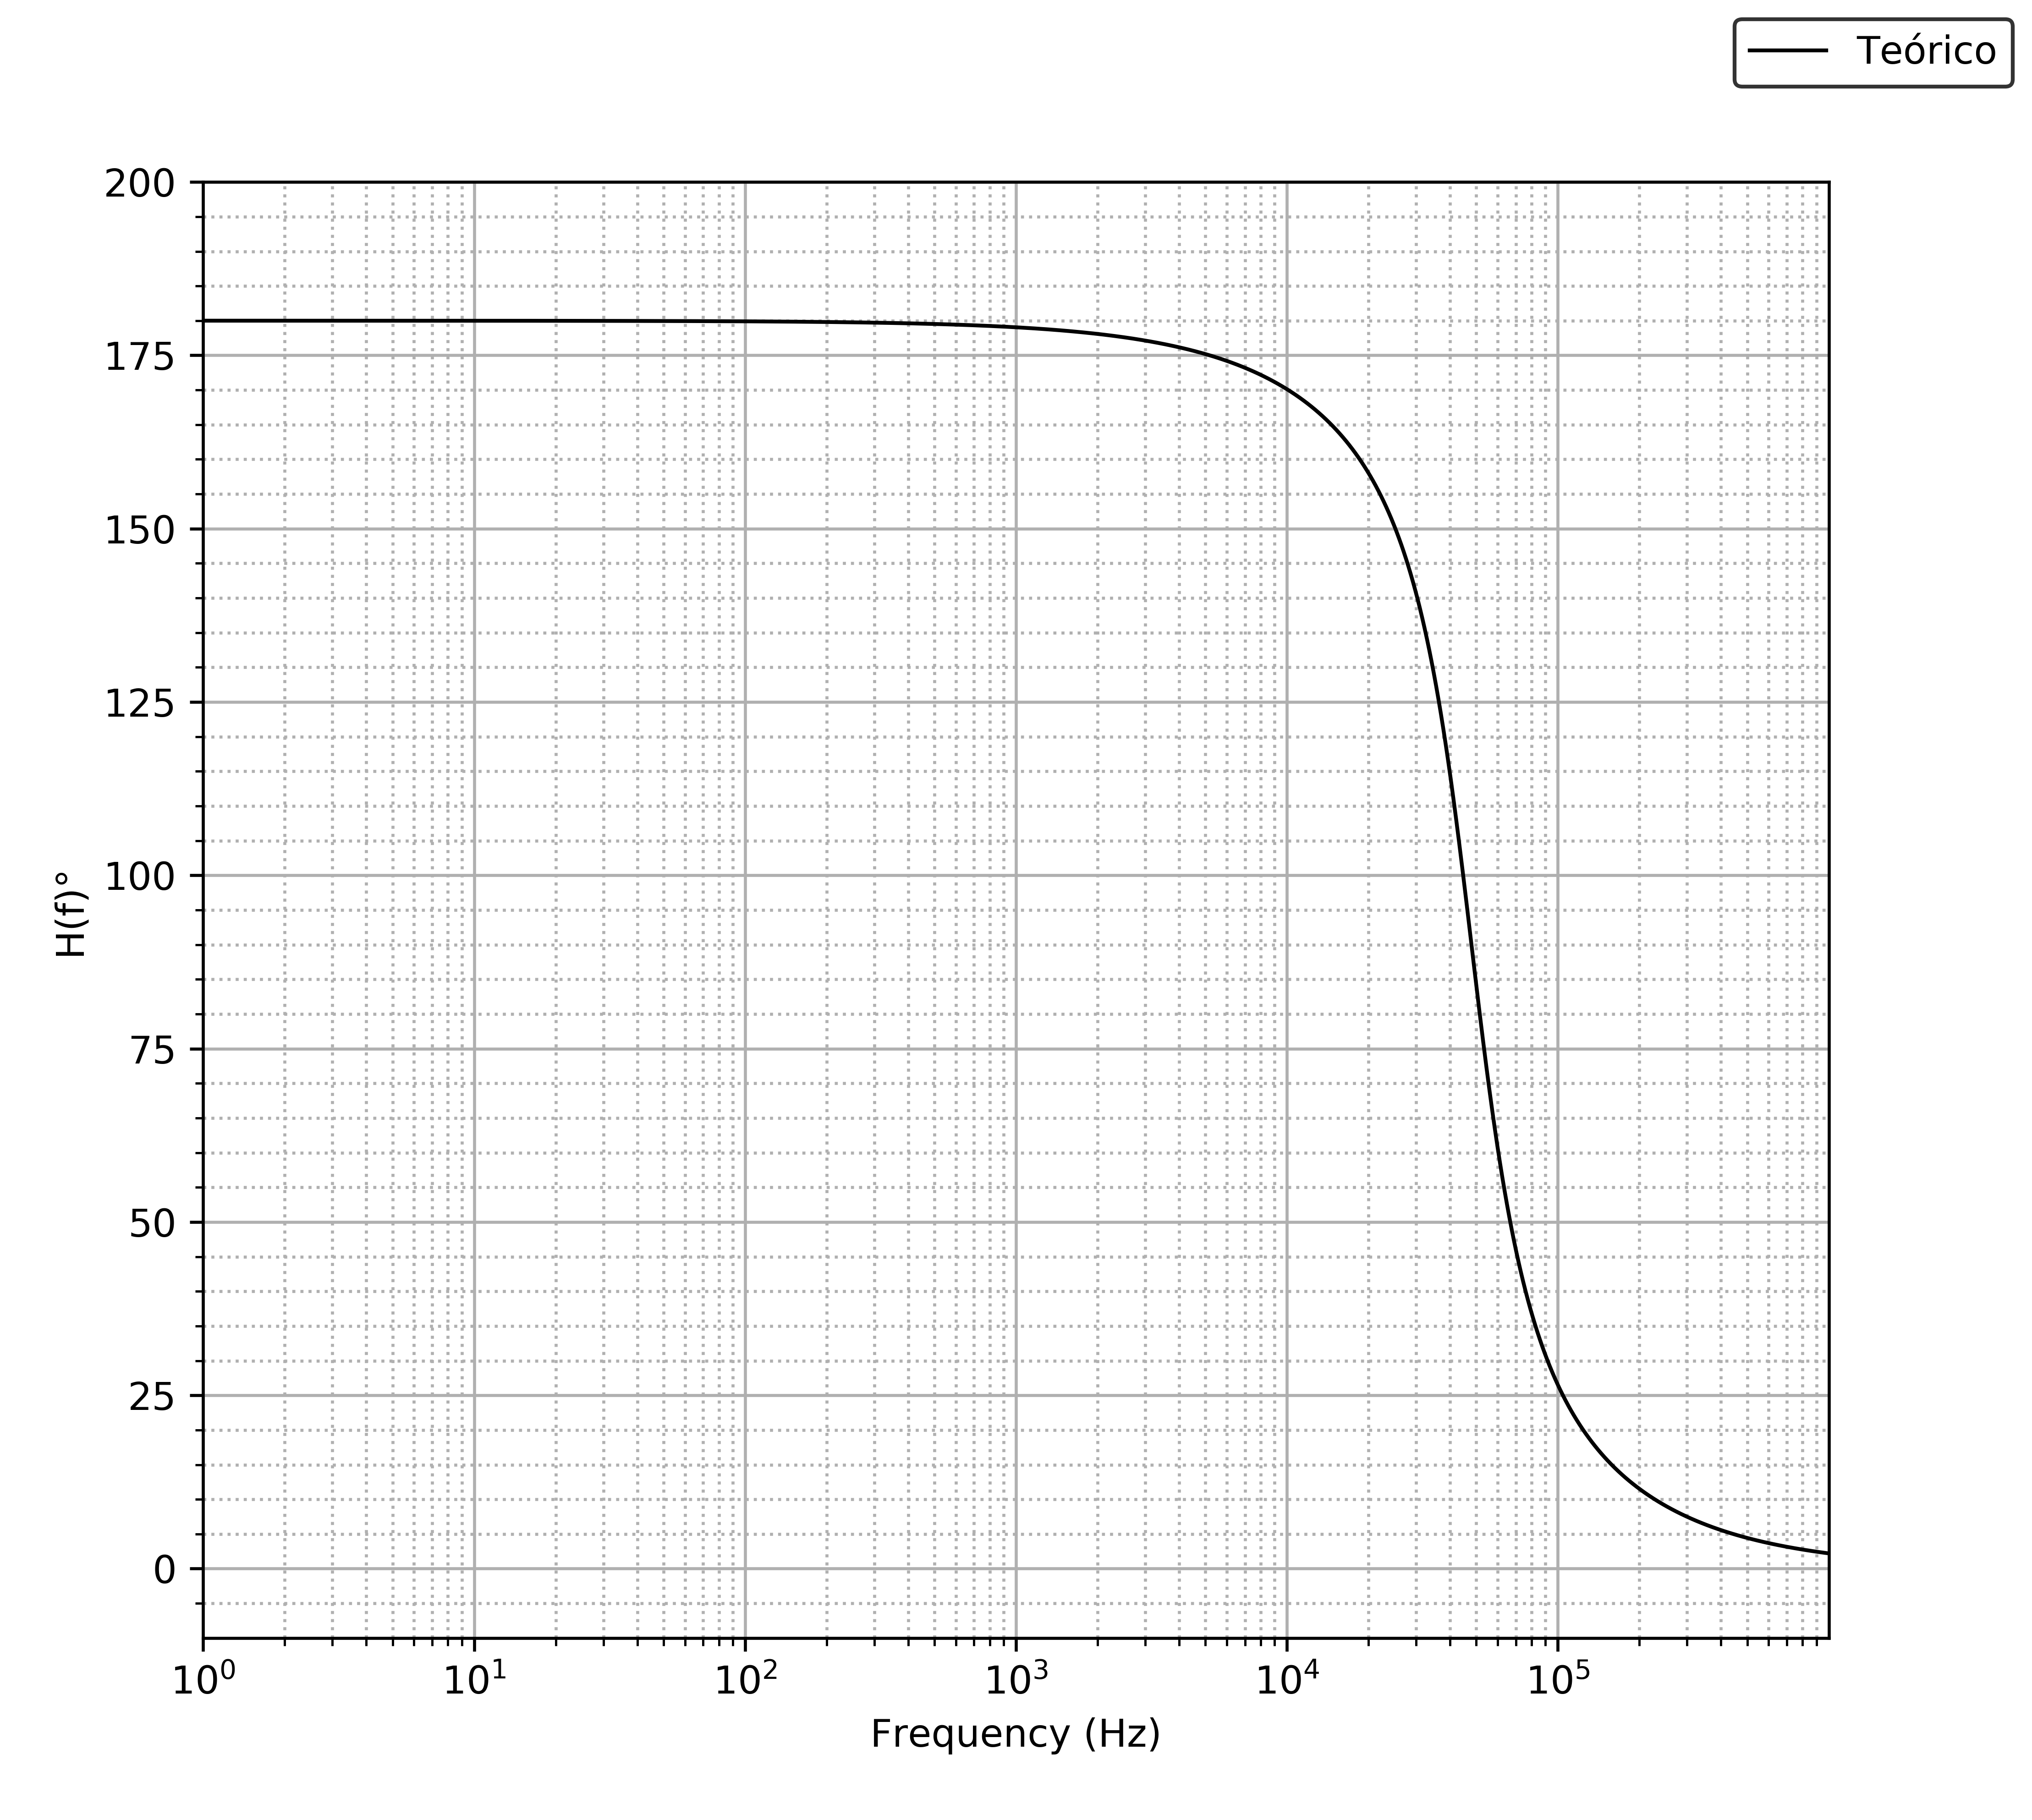
\includegraphics[scale=0.3]{Recursos/bode_teorico_pasaaltos_fase.png}
    \end{tabular}
    \caption{Diagramas de bode te\'orico del circuito pasaaltos}
    \label{fig:bode_pasaaltos_teorico}
\end{figure}

Luego, operando de la forma que se viene haciendo, se excita el circuito con una se\~nal cuadrada para simular un escal\'on de amplitud A,
donde luego la respuesta es:

\begin{equation}
    v_o(t) = \frac{A}{\sqrt{1 - \xi^{2}}} \cdot e^{-\alpha \cdot t} \cdot \sin{(\omega_d \cdot t - \theta)}
\end{equation}

Para este caso de subamortiguamiento, por la forma de la respuesta al escal\'on, para los c\'alculos de tiempo de establecimiento,
tiempo al pico y sobre pico, se pueden reutilizar las expresiones empleadas en el caso del filtro de segundo orden pasabajos, con lo cual
evaluando tales magnitudes, el sistema deber\'a tener el mismo comportamiento en t\'erminos de c\'omo son los valores de dichos par\'ametros.

\begin{table}[H]
    \centering
    \begin{tabular}{c c c c c c c c}
        $R$ & $\xi$ & $t_s$ & $t_p$ & $M_p$ & $Sistema$ \\
        \hline \\
        $120.6 \Omega$ & $0.4$ & $25.56 \mu s$ & $11.368 \mu s$ & $0.253$ & $Subamortiguado$ \\
        \hline
    \end{tabular}
    \caption{Respuesta al escal\'on del pasaaltos}
    \label{tab:tabla_pasaaltos}
\end{table}

\subsubsection{Resultados}

Nuevamente se presentan en primer lugar los resultados correspondientes a la respuesta natural del sistema seguidos de la respuesta en frecuencia del mismo. Antes de exponer dichos resultados, es importante mencionar la complicación que se generó tratando de calibrar la resistencia para lograr el $\xi$ deseado en el cicuito pasaaltos. 

En un principio, se quizo calibrar el valor de la resistencia tal que se lograra un sobrepico determinado lo más cercano posible al valor teórico. Con un potenciómetro se buscó la resistencia deseada, pero se encontró el problema de que tanto la señal de salida como la de entrada se deformaban antes de llegar al valor de $\xi$ estipulado. Se probó cambiando el integrado a otro con menor resistencia de salida, lograndose mejores resultados pero que aún estaban lejos del modelo teórico. Se testeó incluso el circuito sin resistencias, obteniedose así una respuesta oscilatoria. Por último se decidió medir la respuesta en frecuencia con el valor teórico $R = 120 ohm$. El caso anteriormente descrito puede deverse a lo siguiente: debido a que se están midiendo tensiones en una bobina, las cuales son directamente proporcionales al cambio de corriente sobre la misma, es probable que a picos de tensión muy altos la salida del integrado no sea lo suficientemente rápida para seguir los cambios de corriente medidos en la bobina, generado así una curva en la verdadera señal de entrada (después del Buffer) cuya concavidad es opuesta a la respuesta natural del circuito. 

Habiendo explicado la problemática anterior se dejan detallados los parámetros medidos:

\begin{table}[H]
    \centering
    \begin{tabular}{c c c c c}
        $t_s$ & $t_p$ & $M_p$ & $f_o$ & $Sistema$ \\
        \hline \\
        $29.7\mu s$ & $13.6 \mu s$ & $0.27$ & $48,544kHz$ & $Subamortiguado$ \\
        \hline
    \end{tabular}
    \label{tab:natural_pasaaltos}
\end{table}


\begin{figure}[H]
	\centering
	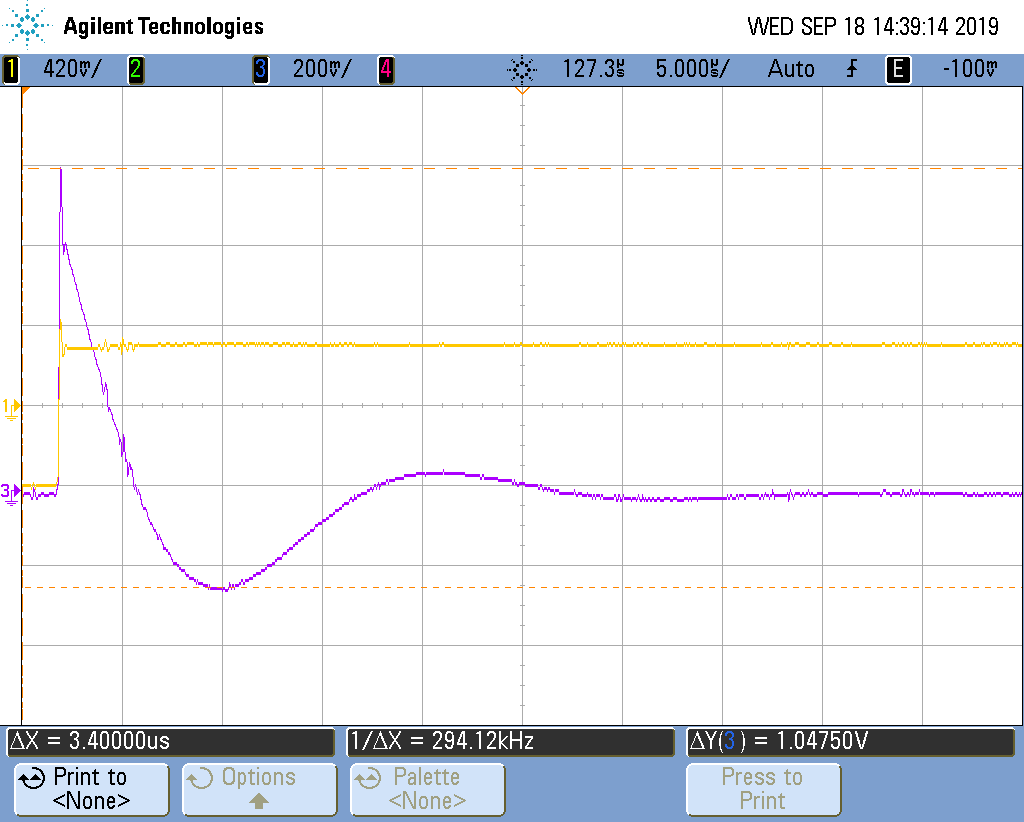
\includegraphics[scale=0.3]{../Mediciones/Osciloscopio/Pasaaltos_respuesta_escalon/scope_4.png}
\end{figure}


De la tabla anterior lo que más llama la atención es la diferencia en cuanto a los tiempos de establecimiento y tiempo al pico de la señal. Tanto para el primero como para el segundo existe un error porcentual mayor al 20 porciento. Es de esperarse que los resutlados teóricos y empíricos no concuerden teniendo en cuenta el problema en la calibración que se detalló anteriormente. Un tiempo de establecimiento mayor significa que el valor de la resistencia no era lo suficientemente grande para llegar al valor de $\xi$ deseado.


A continuación se presenta la respuesta en frecuencia del circuito:

\begin{figure}[H]
    \centering
    \begin{tabular}{c c}
        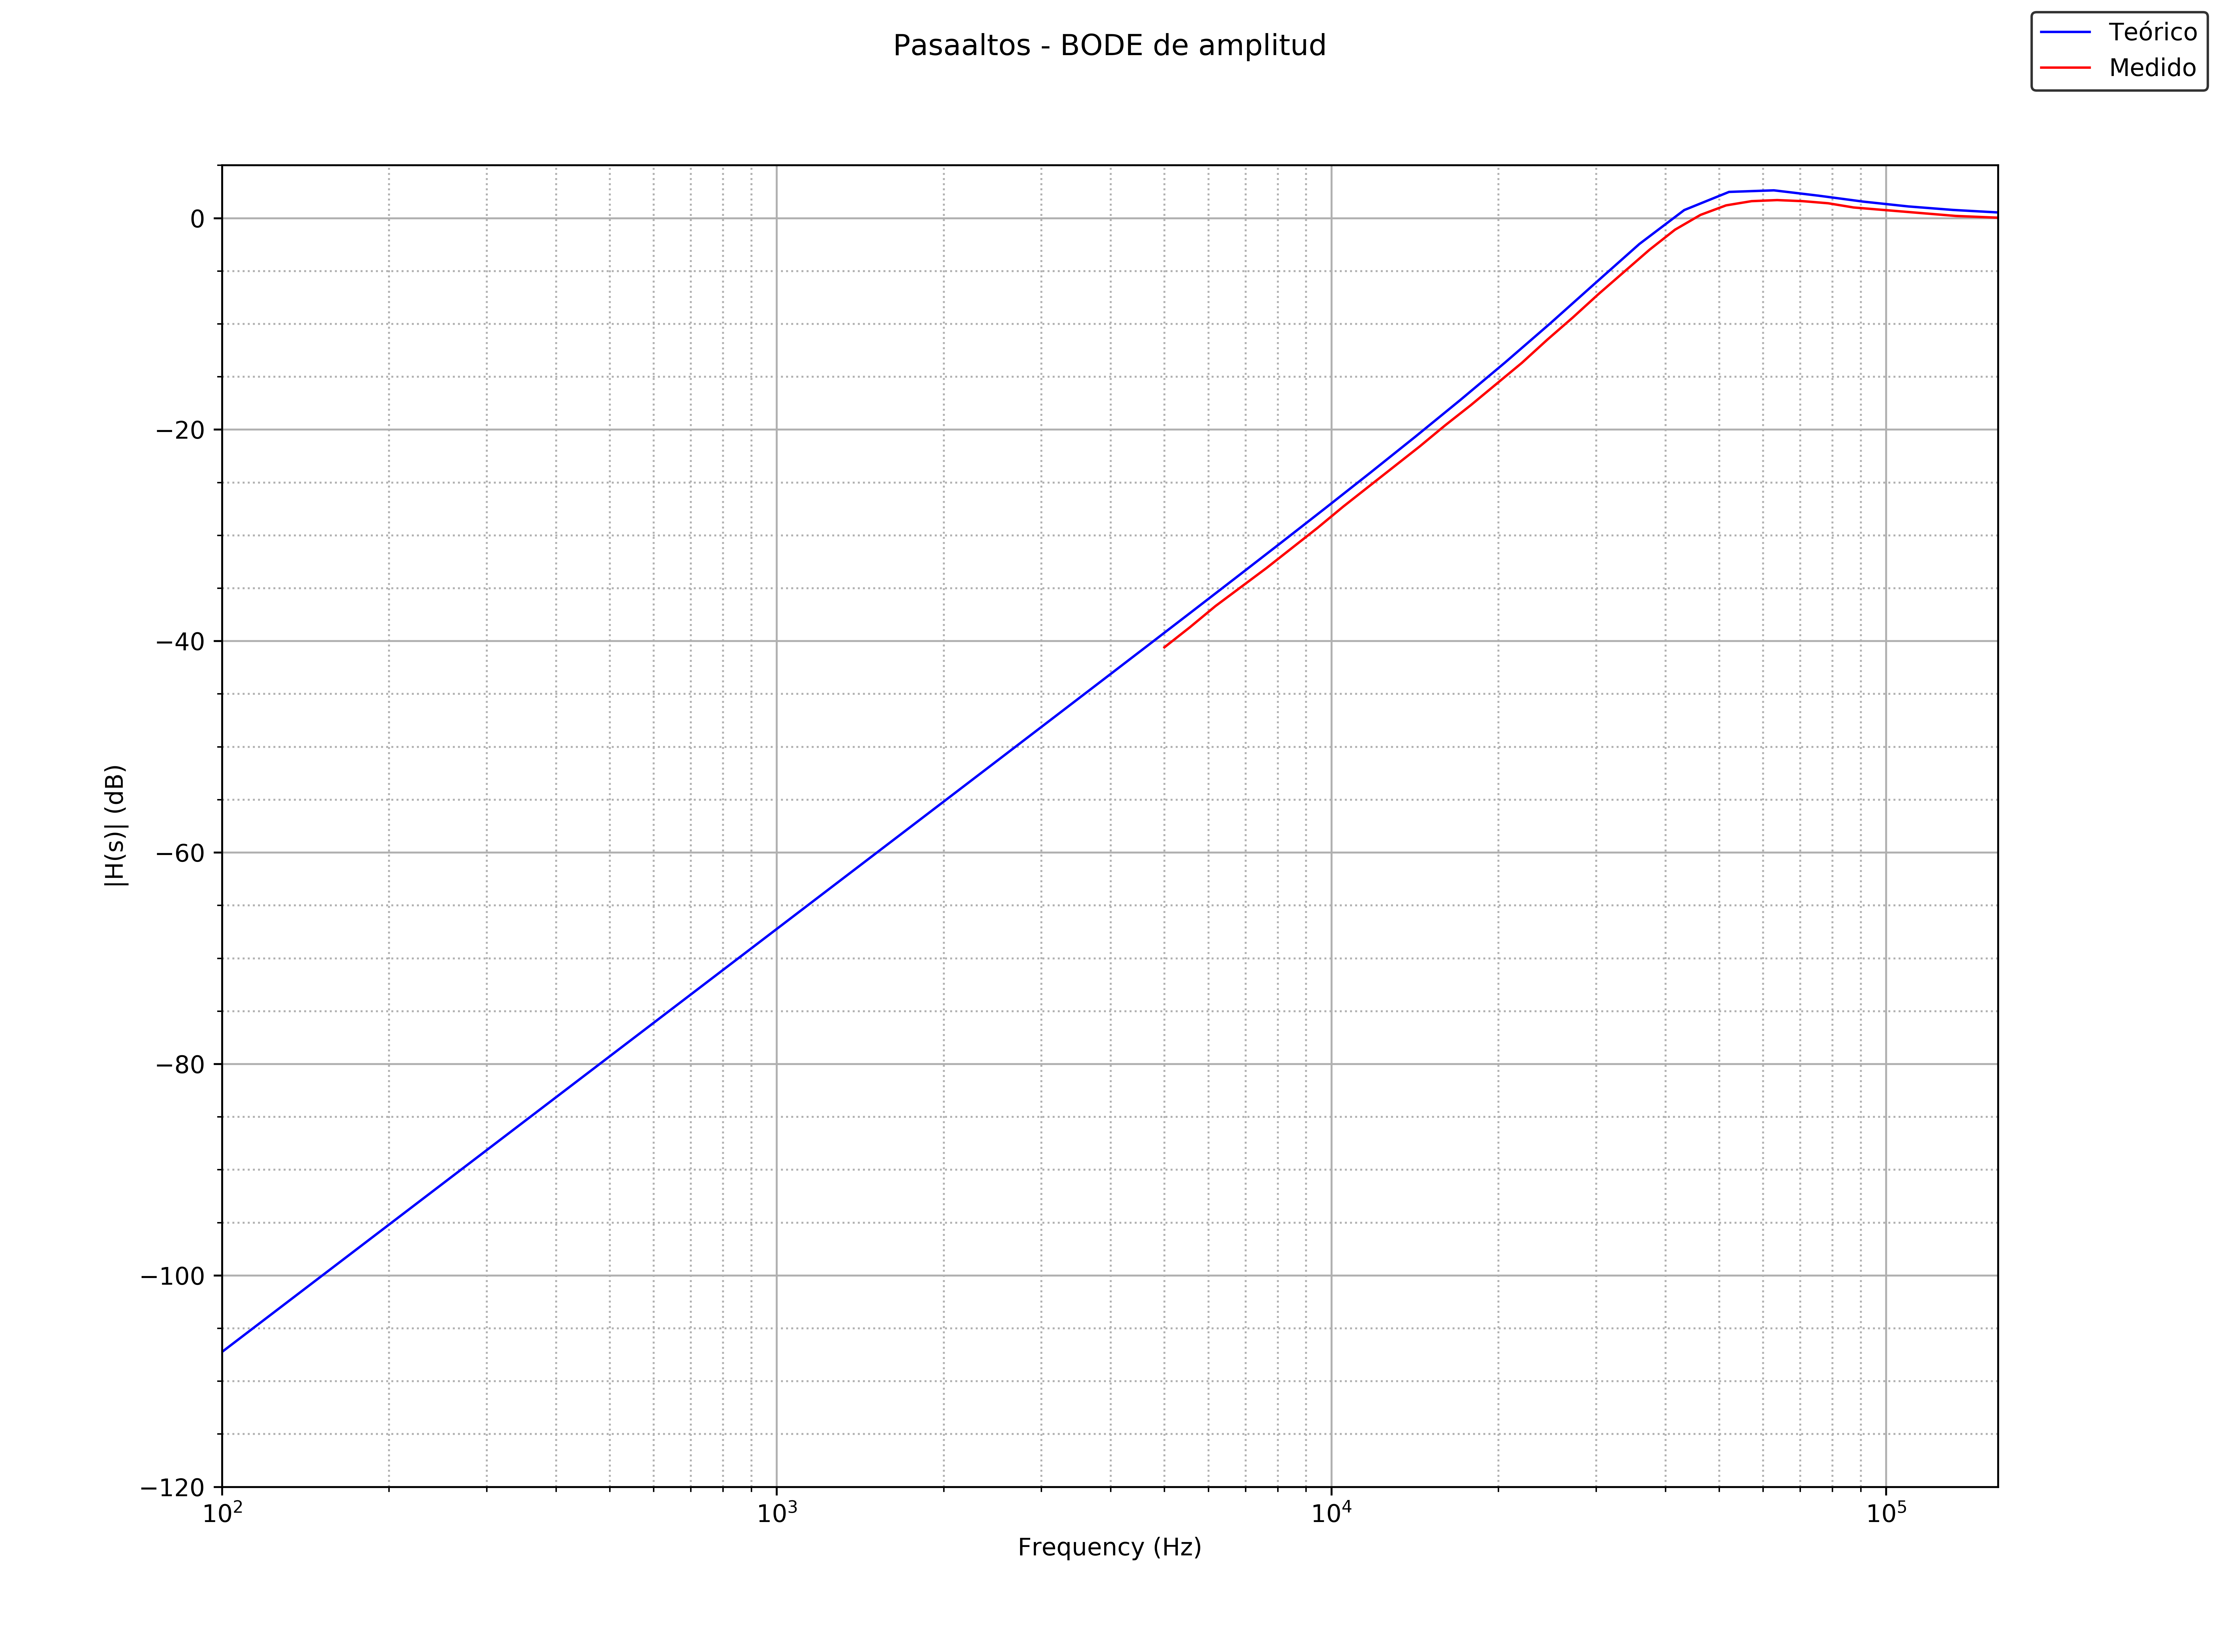
\includegraphics[scale=0.3]{Recursos/ej4/pasaaltos_amplitud.png}
        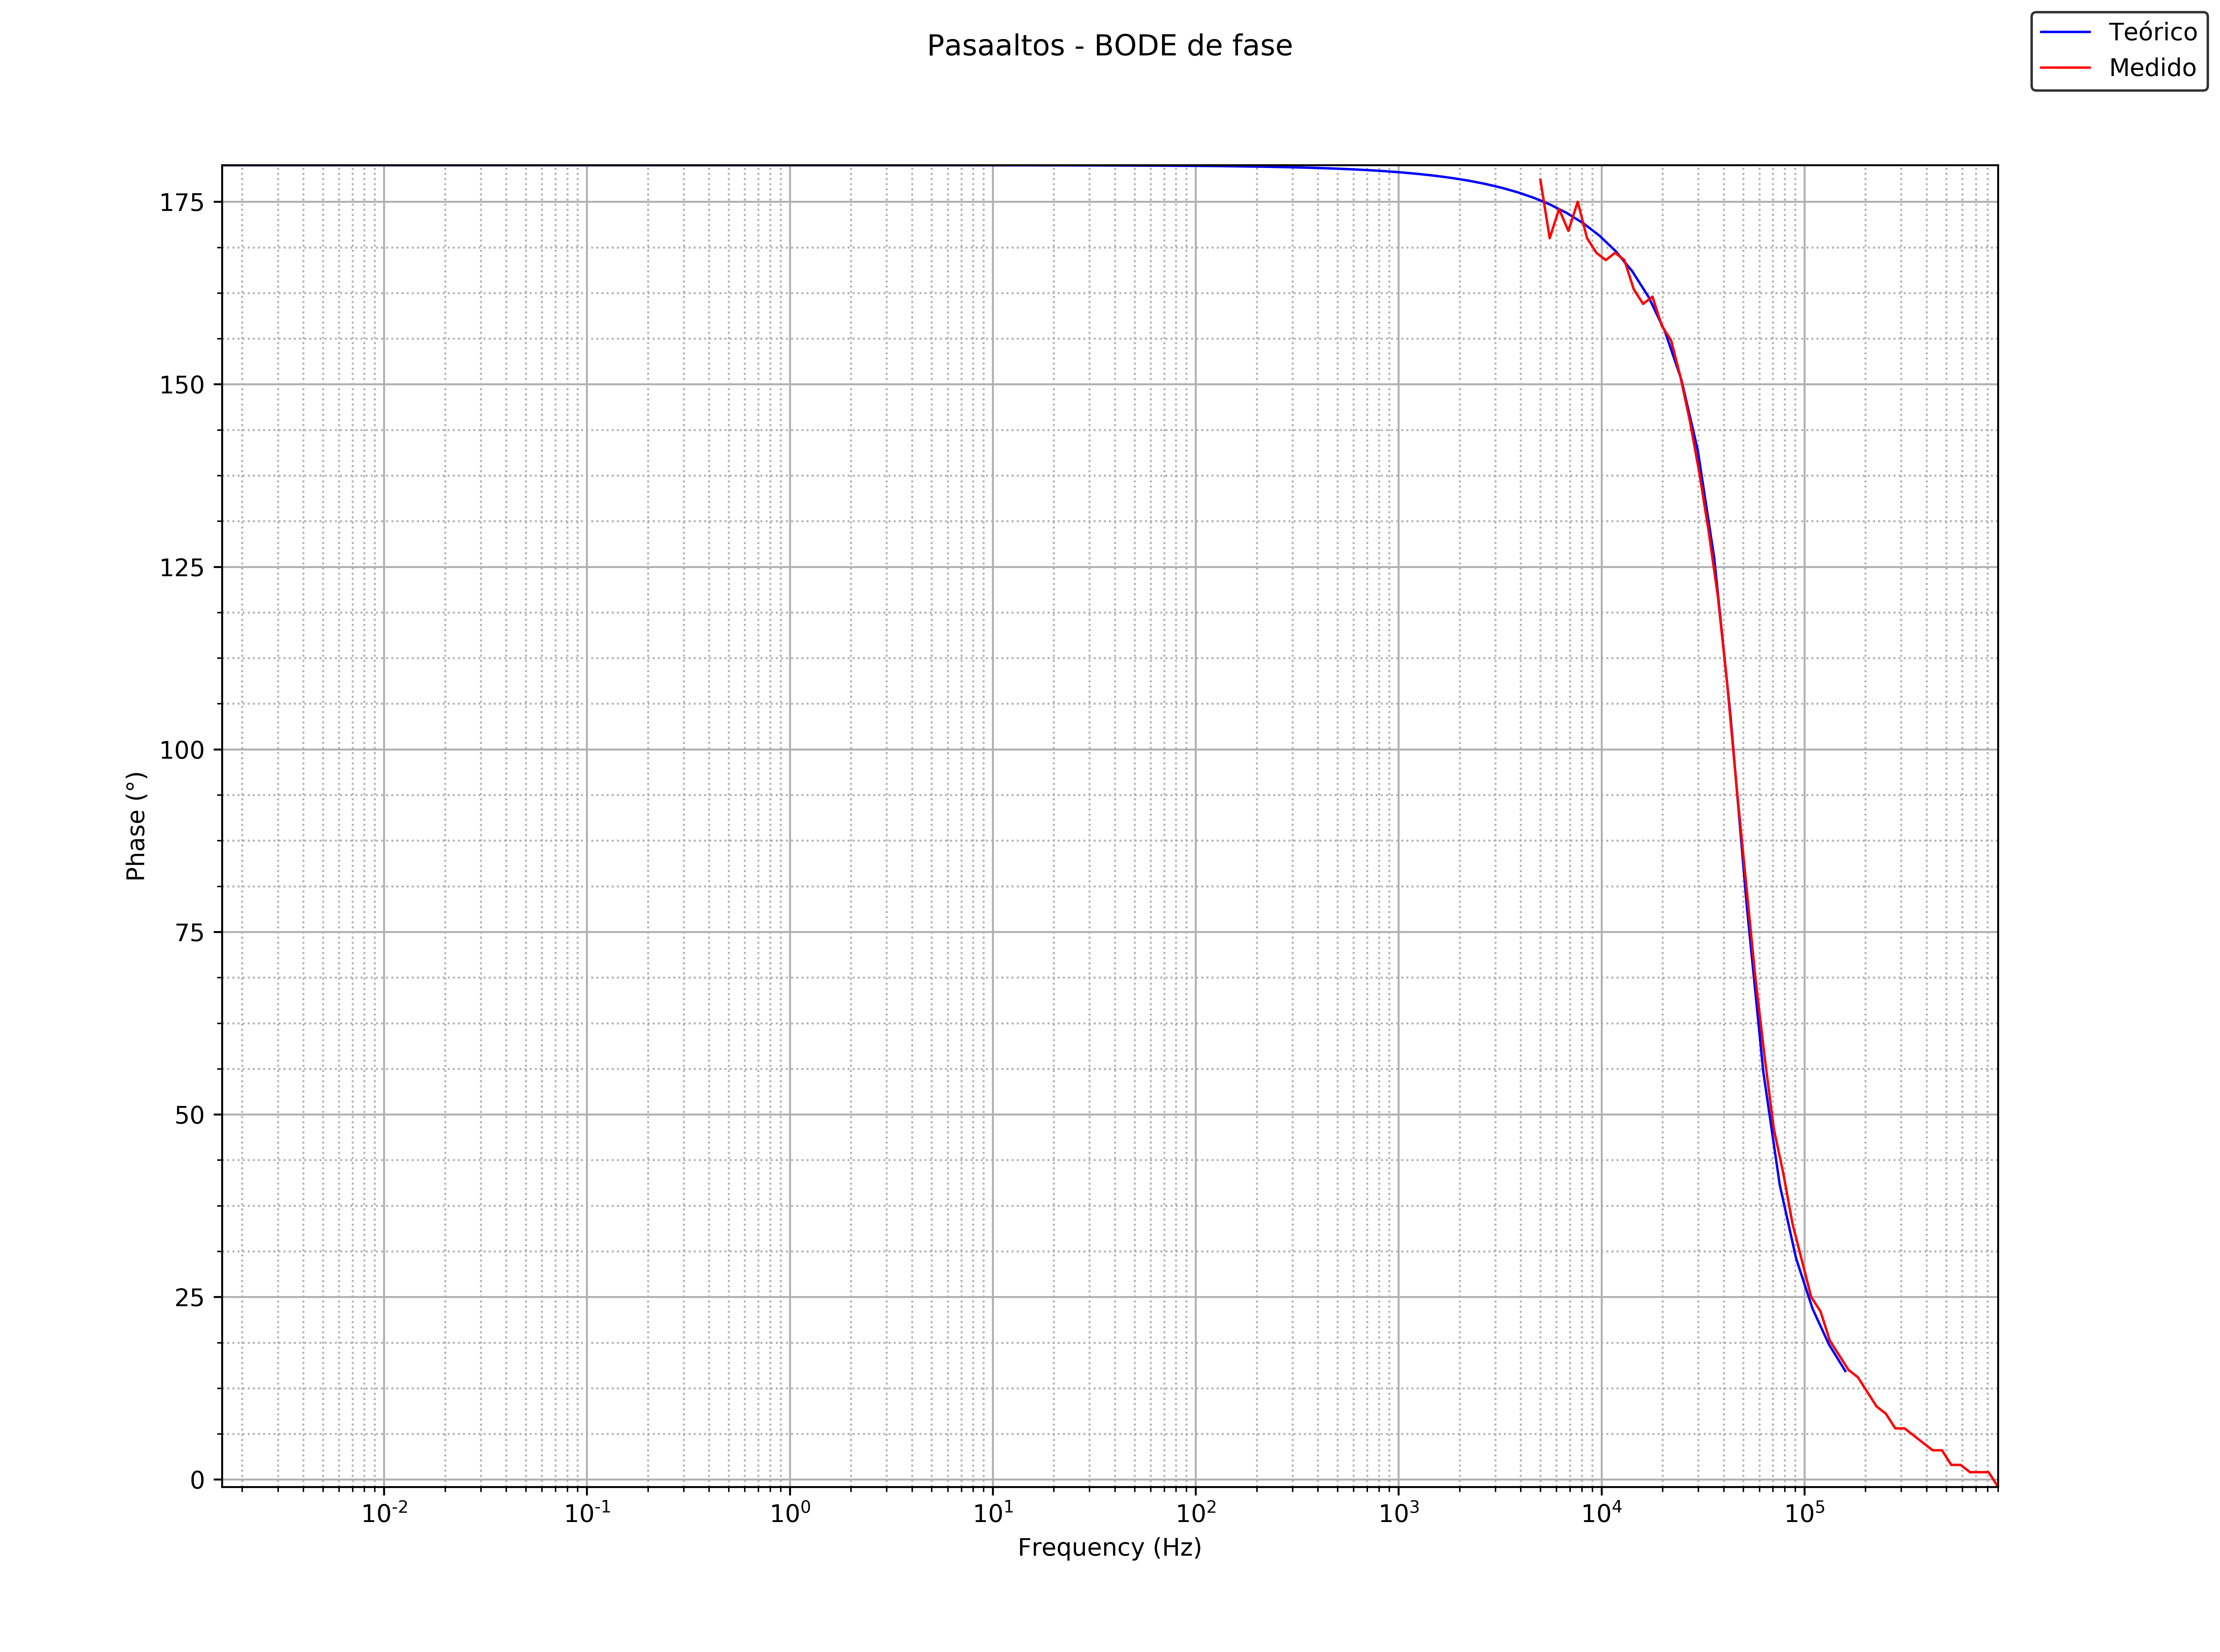
\includegraphics[scale=0.3]{Recursos/ej4/pasaaltos_fase.png}
    \end{tabular}
    \caption{Diagramas de bode teóricos frente a medidos pasaaltos}
    \label{fig:bode_pasaaltos_comparacion}
\end{figure}

Para el gráfico en amplitud del circuito pasaaltos se obtuvo una curva que concuerda en gran medida con el caso teórico ideal. No obstante lo anterior, salta a la vista que no hay mediciones menores a los $3kHz$. La atenuación a esas frecuencias es superior a los $40dB$ y se midieorn señales con amplitudes menores a los $20mV$, por lo que discernir entre ruido y la señal de salida fue imposible. Para el caso de la fase ocurre algo similar. La curva se comporta acorde al modelo teorizado excepto a bajas frecuencias, para las cuales fue difícil obtener una medición de fase precisa. En cocnlusión, a pesar de las diferencias obtenidas en la respuesta natural del circuito y las dificultades para su calibración, las mediciones en el plano de las frecuencias concuerdan con lo esperado de un filtro con estas características.

\subsection{Circuito Rechazabanda}

\begin{figure}[H]
    \centering
    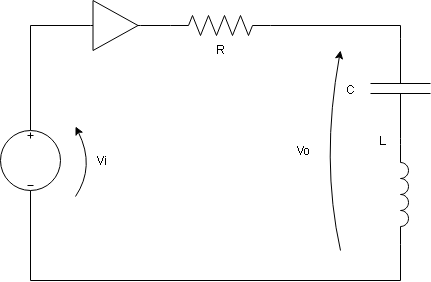
\includegraphics[scale=0.5]{Recursos/circuito_notch.png}
    \caption{Circuito rechazabanda}
    \label{fig:circuito_rechazabanda}
\end{figure}

\subsubsection{An\'alisis te\'orico}
Realizando el mismo desarrollo que se viene haciendo para encontrar la funci\'on transferencia y reutilizando las definiciones de los par\'ametros,
se obtiene que:

\begin{eqnarray}
    H(s) = \frac{\left(\frac{s}{\omega_o} \right)^{2} + 1}{\left(\frac{s}{\omega_o} \right)^{2} + s \cdot \frac{2 \cdot \xi}{\omega_o} + 1}
\end{eqnarray}

Esta \'ultima expresi\'on tiene un cociente de polinomios cuadr\'aticos, que como tales, al caracterizarlos a trav\'es de los par\'ametros que se vienen utilizando
se observa que se presentan dos ceros complejos y conjugados y dos polos complejos y conjugados, particularmente los ceros son de transmisi\'on y ambas partes poseen la misma 
frecuencia de corte. Esto \'ultimo implica que en verdad la respuesta en frecuencia del circuito tiene un comportamiento que no aten\'ua en casi ninguna frecuencia, salvo en torno a tal frecuencia
de corte, por eso se llama rechaza banda.

\begin{figure}[H]
    \centering
    \begin{tabular}{c c}
        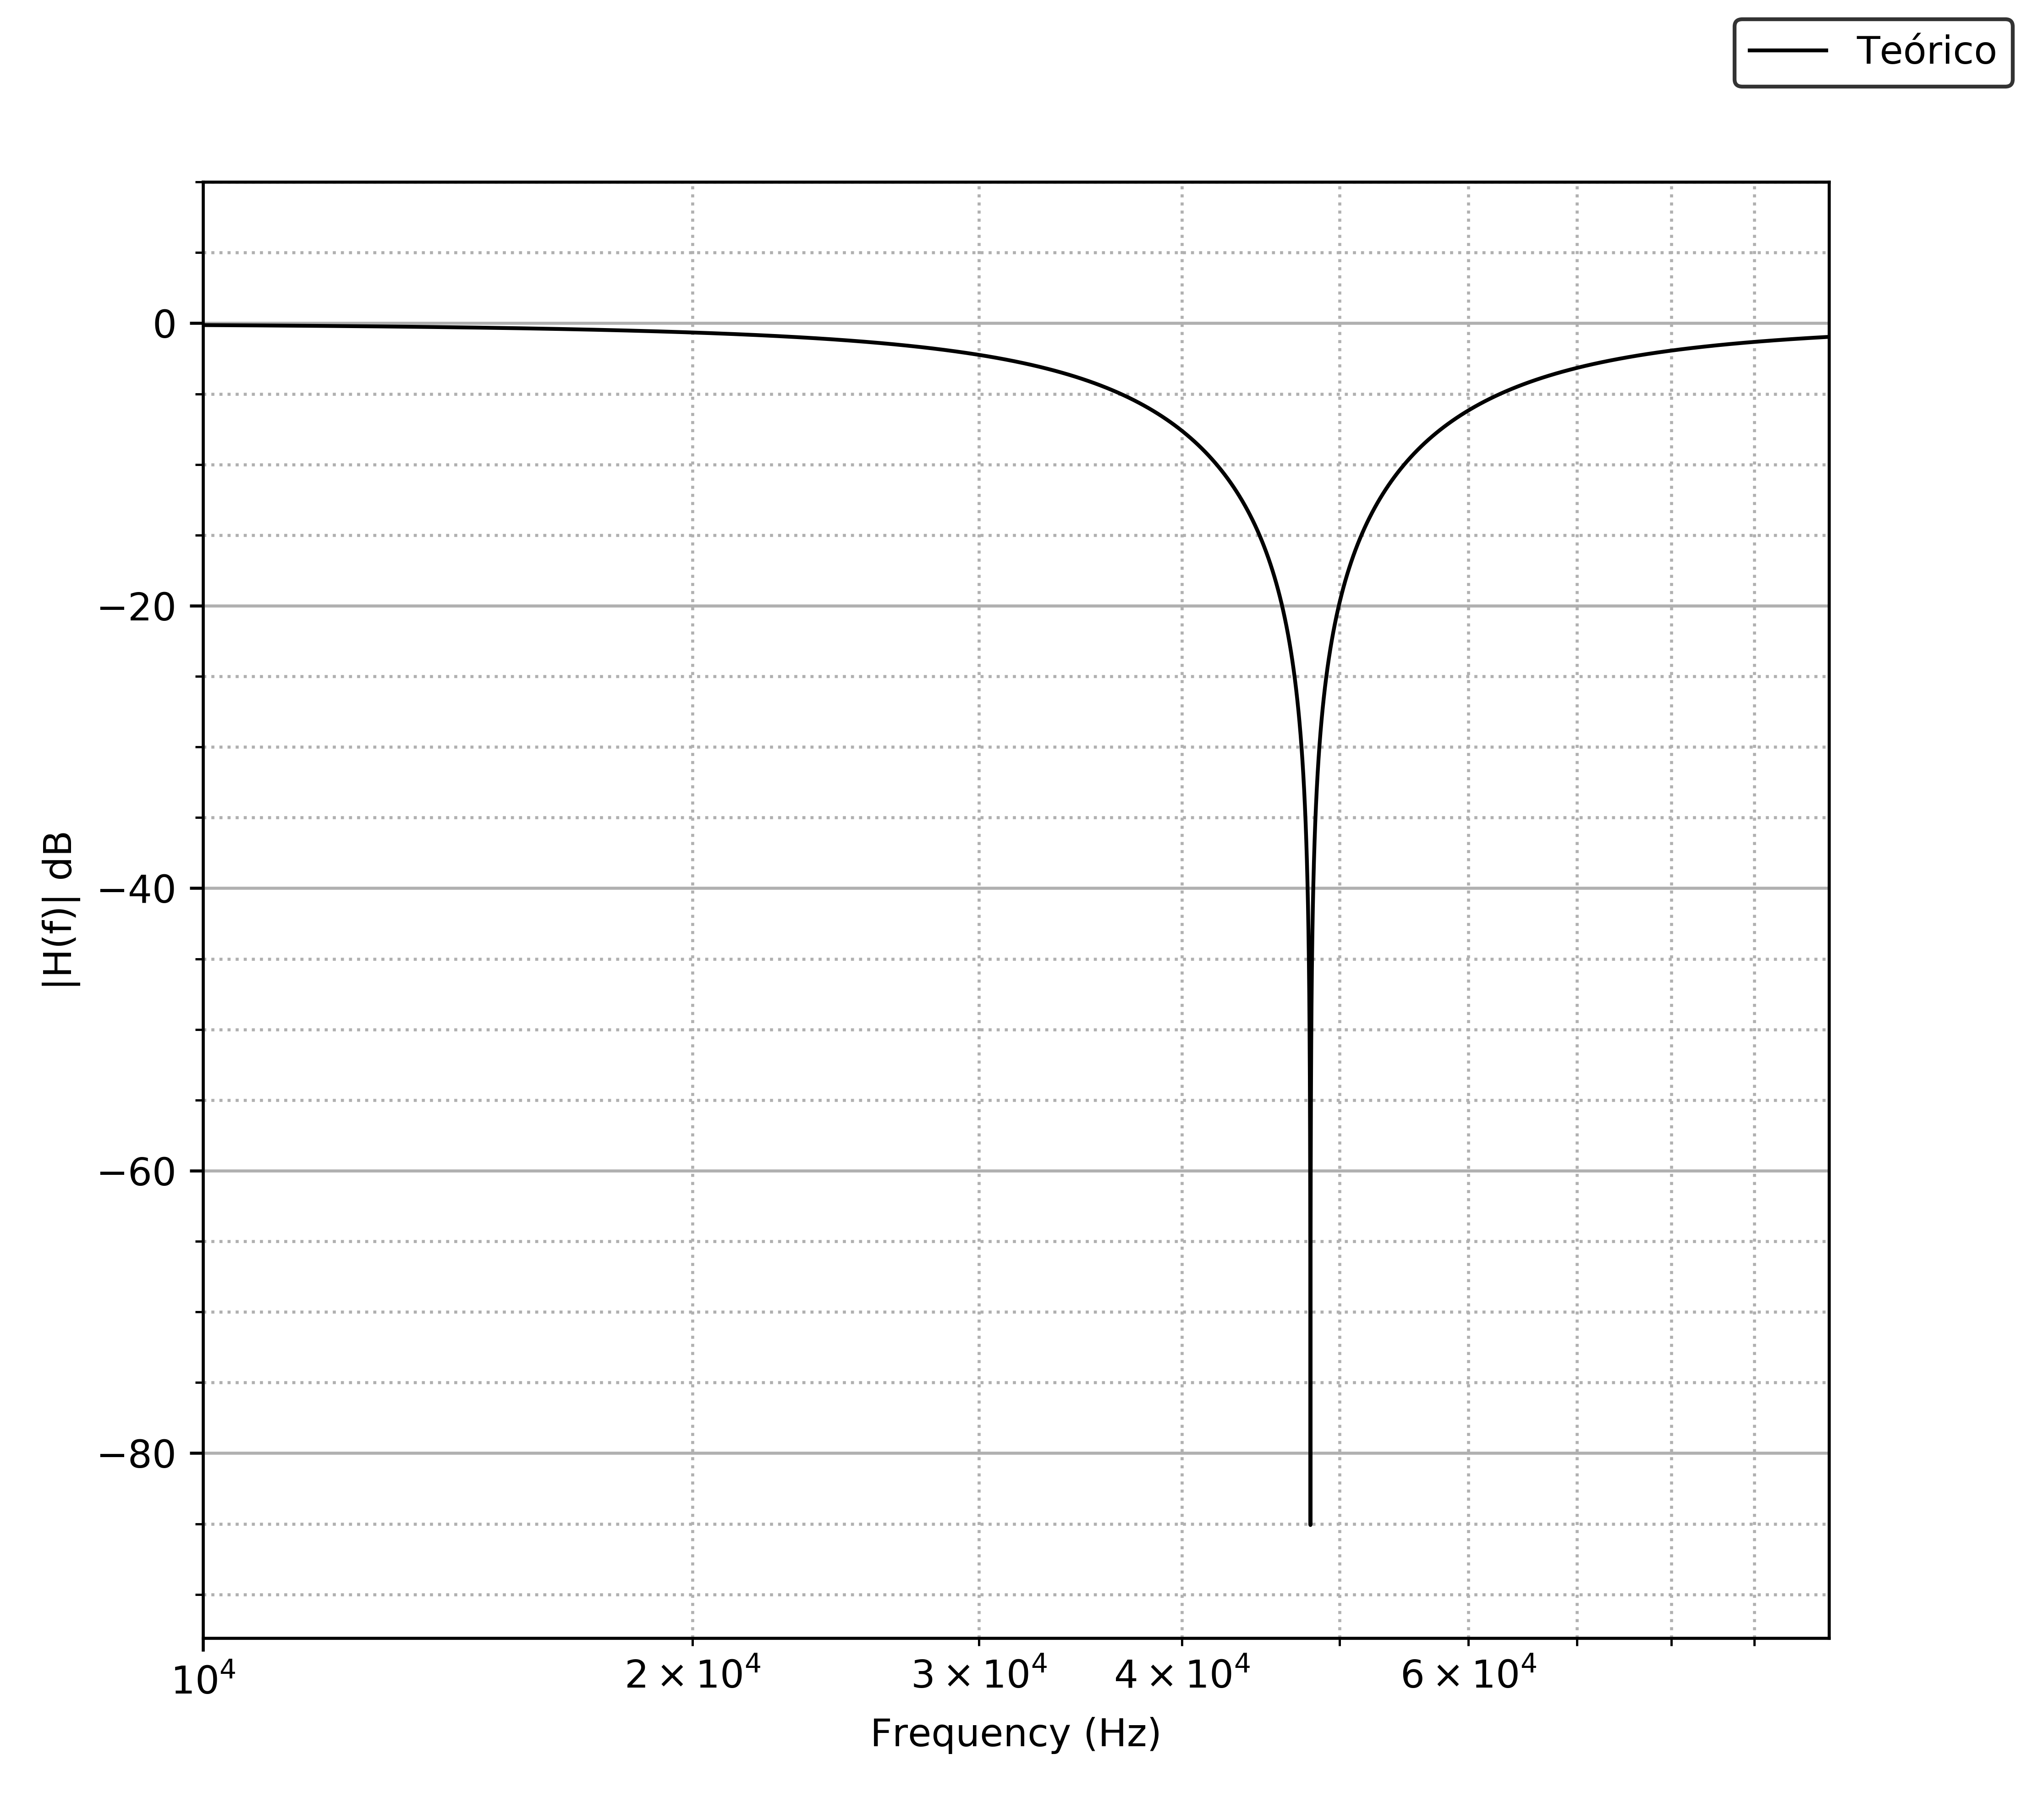
\includegraphics[scale=0.4]{Recursos/bode_teorico_rechazabanda_modulo.png}
        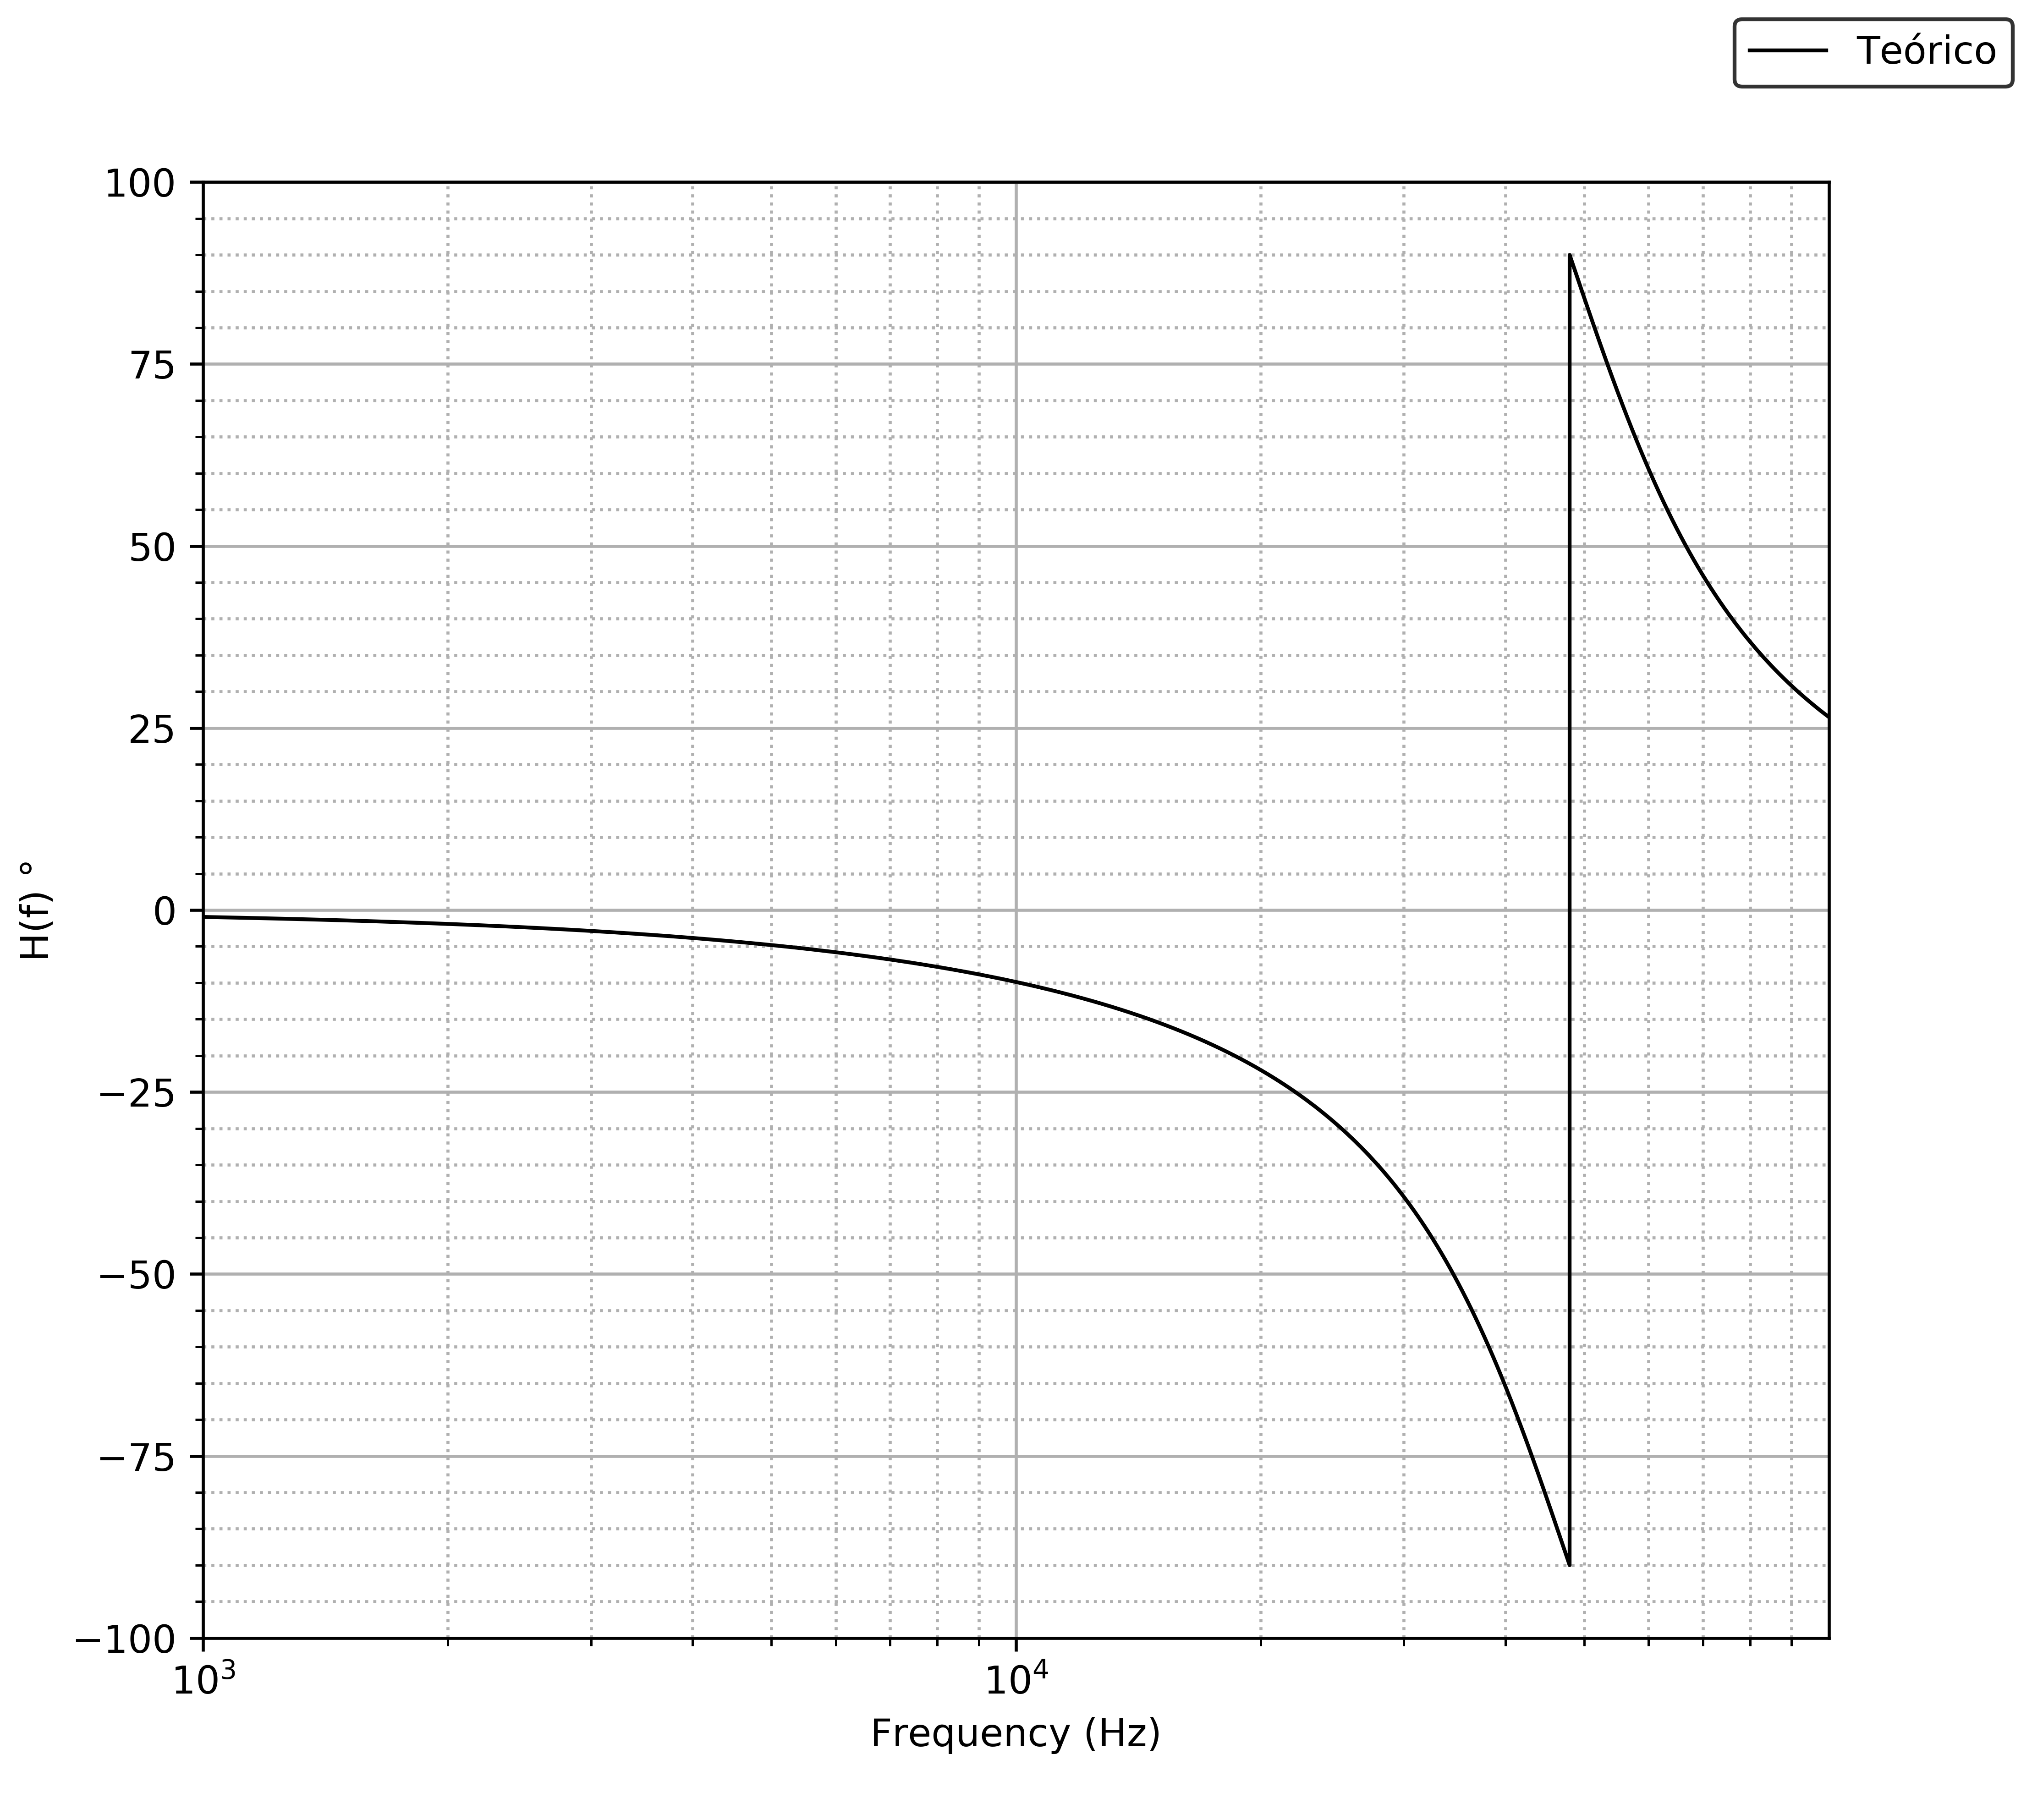
\includegraphics[scale=0.4]{Recursos/bode_teorico_rechazabanda_fase.png}
    \end{tabular}
    \caption{Diagramas de bode te\'orico del circuito rechazabanda}
    \label{fig:bode_rechazabanda_teorico}
\end{figure}

Para no tener que realizar los c\'alculos nuevamente, dado que no ser\'ia necesario, si se busca la respuesta al escal\'on por como est\'a dado el circuito,
lo \'unico que debe hacerse es sumarse las tensiones correspondientes a los casos de un filtro de segundo orden pasabajos y pasaltos, y en ese caso se obtiene
reutilizando las expresiones encontradas en esos an\'alisis te\'oricos.

\begin{equation}
    v_o(t) = A - \frac{A \cdot e^{-\alpha \cdot t} }{\sqrt{1 - \xi^{2}}} \cdot \sin{\omega_d \cdot t} \left( 2 \cdot \xi -1 \right)
\end{equation}

De donde luego se despejan las expresiones:

\begin{equation}
    t_p = \frac{\arctan{\frac{\sqrt{1 - \xi^{2}}}{\xi}}}{\sqrt{1 - \xi^{2}} \cdot \omega_0}
\end{equation}

\begin{equation}
    t_s = \frac{ \ln{(\frac{0.05 \cdot \sqrt{1 - \xi^{2}}}{2 \cdot \xi})} }{- \xi \cdot \omega_o}
\end{equation}


La expresi\'on de $M_p$ sale de reemplazar $t_p$ dentro de la ecuaci\'on $v_o(t)$.

\begin{table}[H]
    \centering
    \begin{tabular}{c c c c c c c c}
        $R$ & $\xi$ & $t_s$ & $t_p$ & $M_p$ & $Sistema$ \\
        \hline \\
        $120.6 \Omega$ & $0.4$ & $4.195 \mu s$ & $25.56 \mu s$ & $0.12$ & $Subamortiguado$ \\
        \hline
    \end{tabular}
    \caption{Respuesta al escal\'on del rechazabanda}
    \label{tab:tabla_rechazabanda}
\end{table}

\subsubsection{Resultados}
Para este circuito se emplearon los mismos componentes del pasaaltos y rechazabanda, sin realizar una calibraci\'on adicional del $\xi$ dado que se realiz\'o para los casos anteriores.

Se someti\'o el circuito a una se\~nal cuadrada peri\'odica, de forma tal de emular un escal\'on y poder medir la respuesta natural del sistema al mismo, que se presenta a continuaci\'on.

\begin{figure}[H]
	\centering
	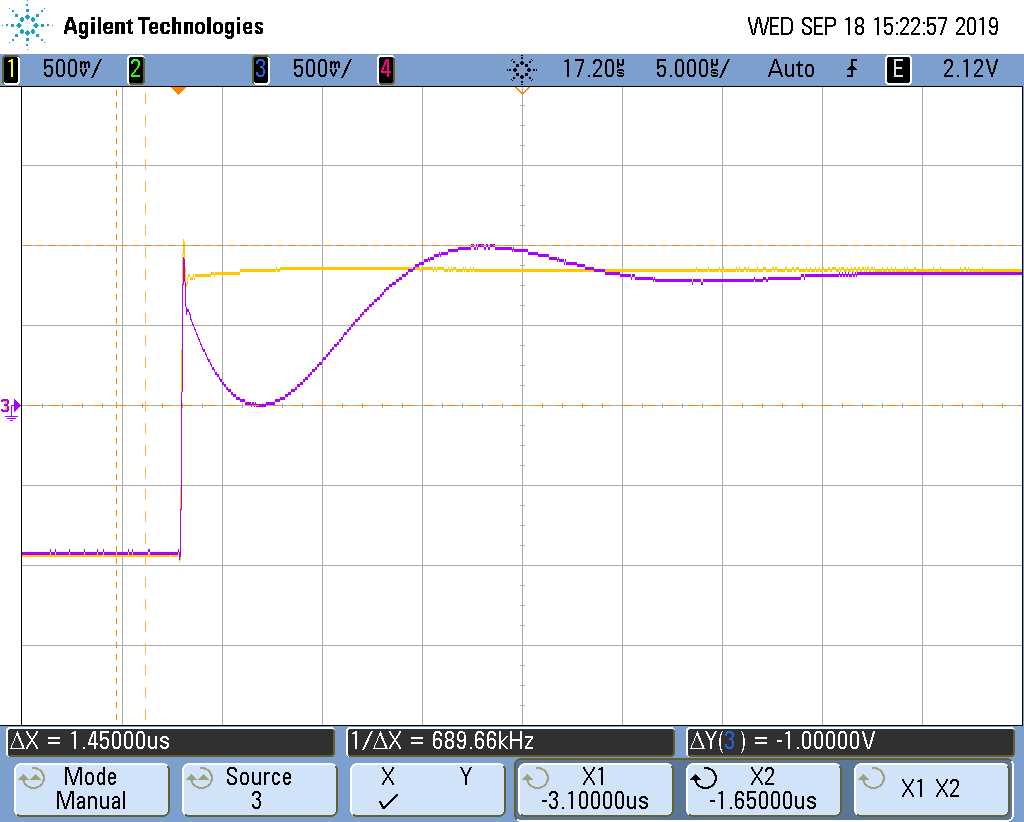
\includegraphics[scale=0.3]{../Mediciones/Osciloscopio/Rechazabanda_respuesta_escalon/scope_5.png}
\end{figure}

Por otro lado, se reproducen las mediciones realizadas sobre esta respuesta:

\begin{table}[H]
    \centering
    \begin{tabular}{c c c c c}
        $t_s$ & $t_p$ & $M_p$ & $f_o$ & $Sistema$ \\
        \hline \\
        $37 \mu s$ & $21 \mu s$ & $0.111$ & $67,34kHz$ & $Subamortiguado$ \\
        \hline
    \end{tabular}
    \label{tab:natural_rechazabanda}
\end{table}



Adem\'as se realizaron las mediciones correspondientes a la respuesta en frecuencia del circuito. A continuaci\'on se encuentran dichos resultados, superpuestos con las curvas te\'oricas de forma tal de tener una referencia.

\begin{figure}[H]
	\centering
	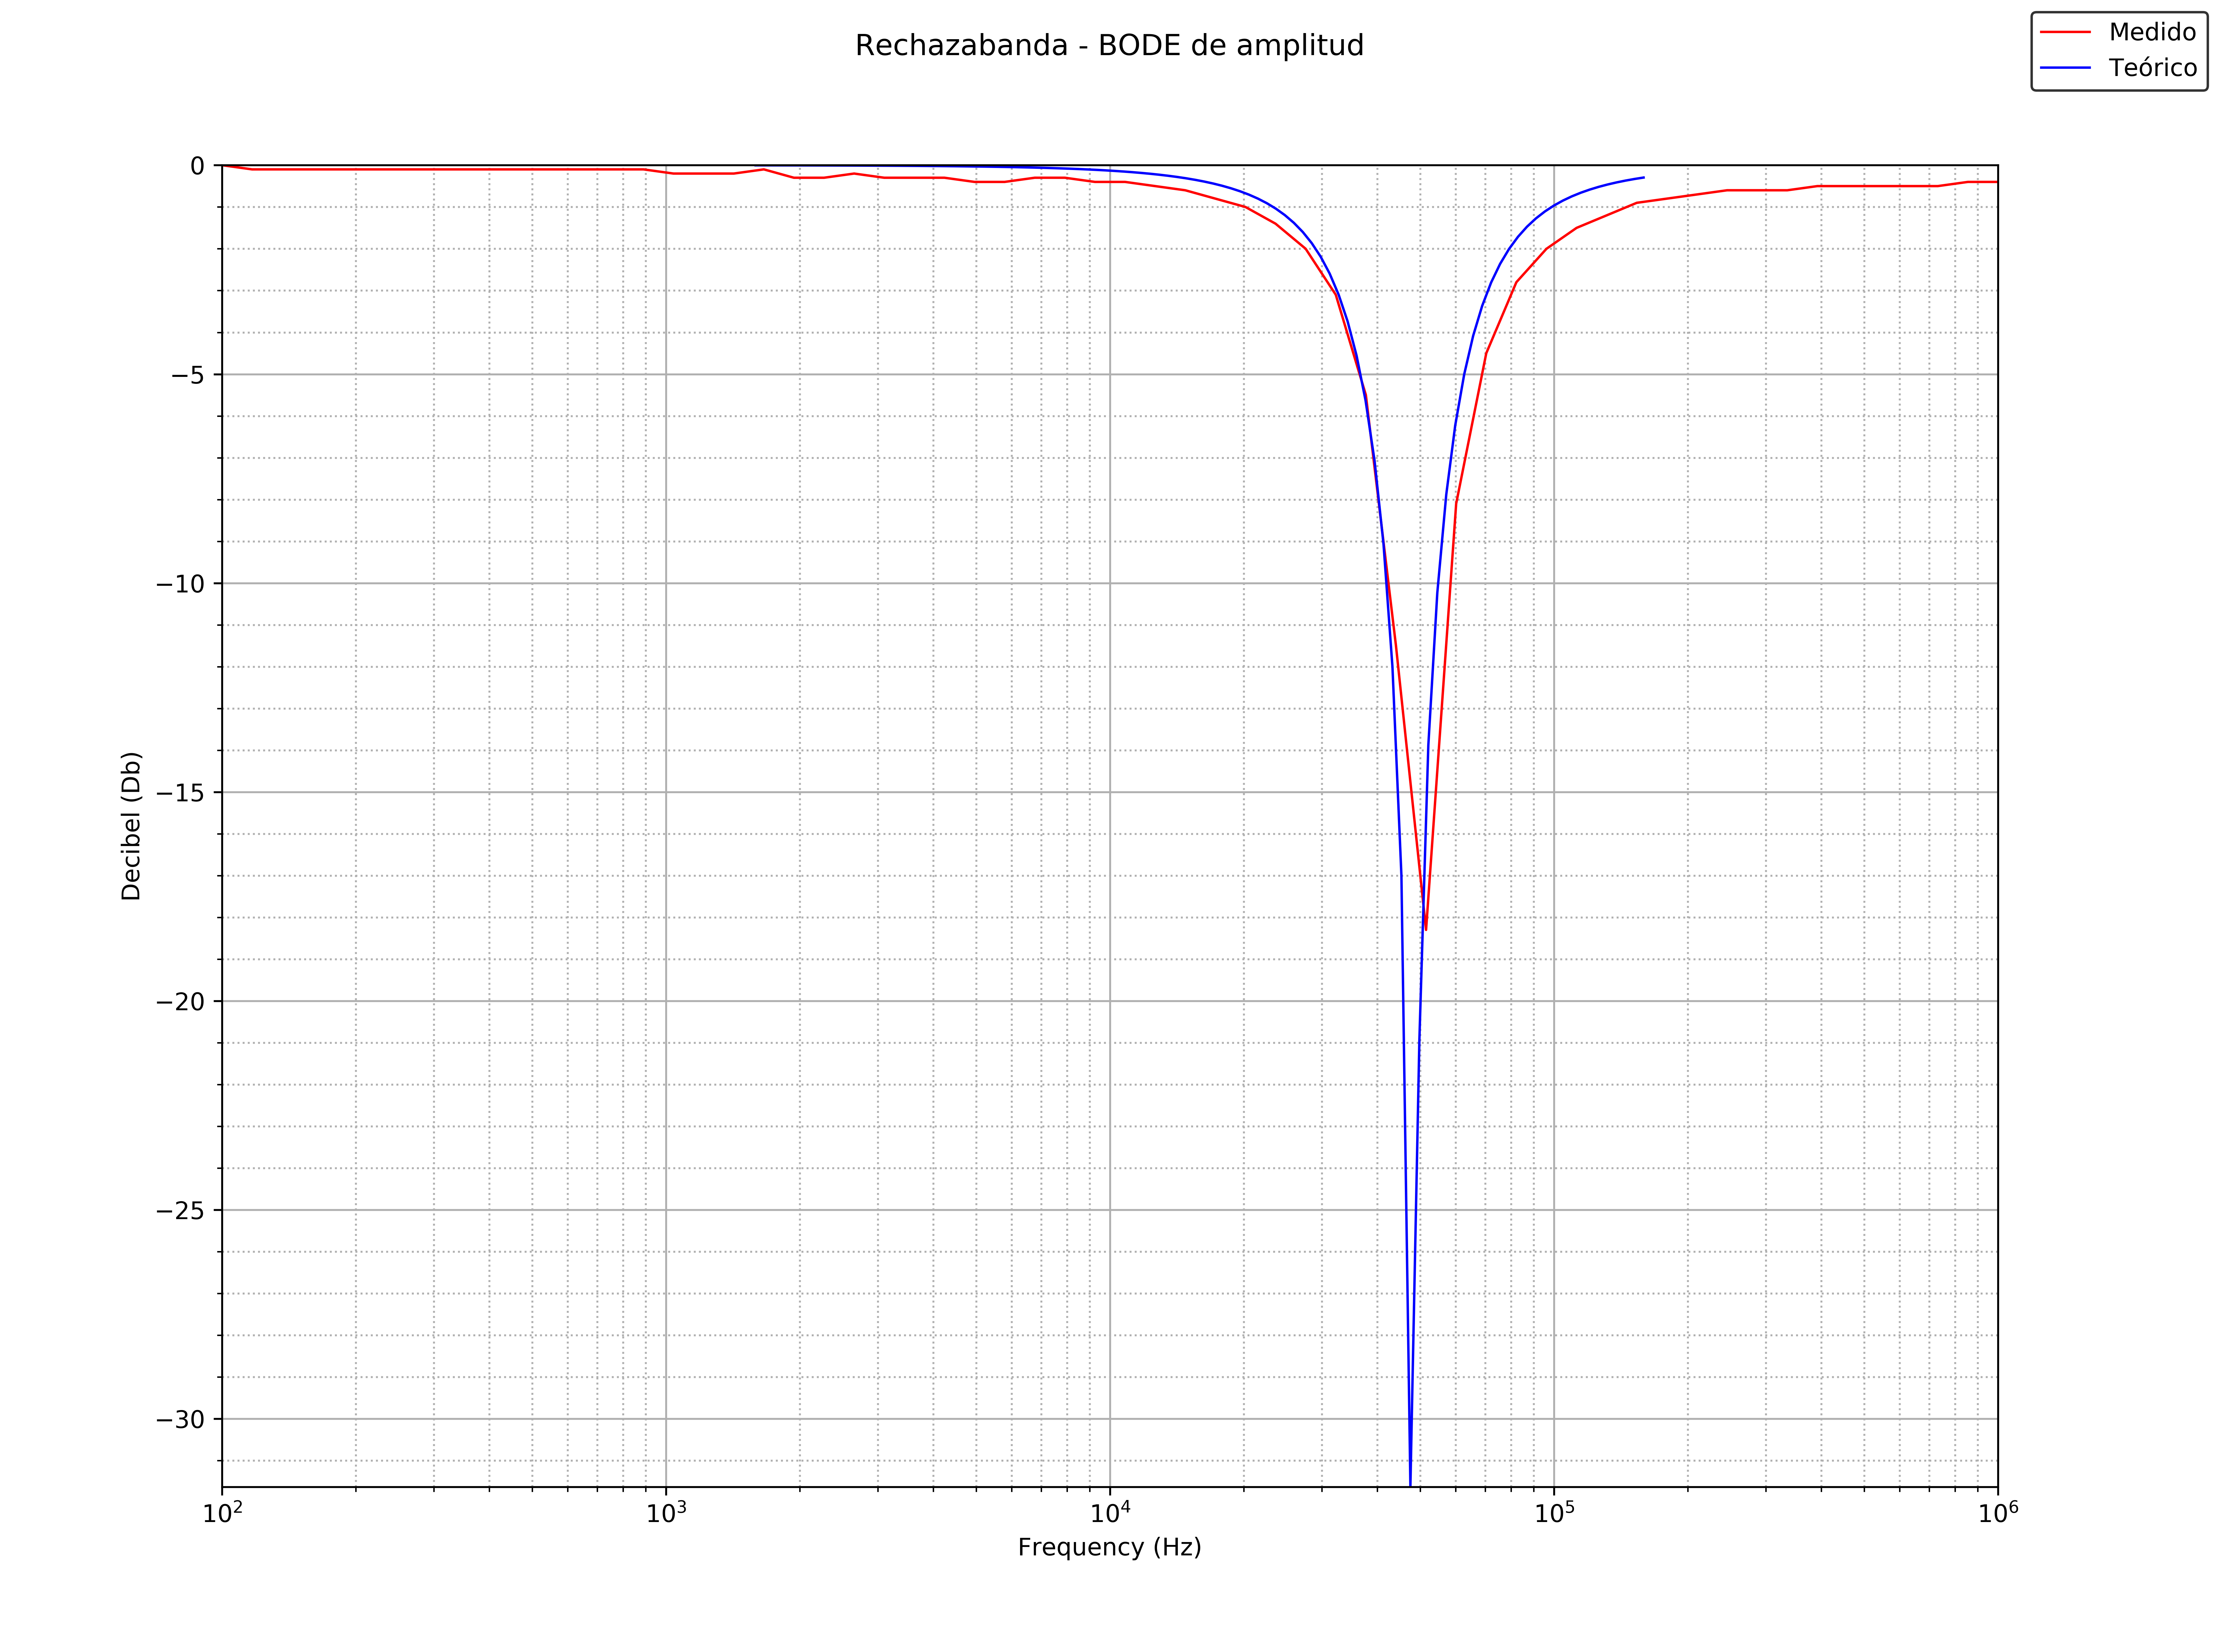
\includegraphics[scale=0.3]{./Recursos/ej4/rechazabanda_amplitud.png}
	\caption{Diagrama BODE de amplitud - Circuito rechazabanda}
\end{figure}

\begin{figure}[H]
	\centering
	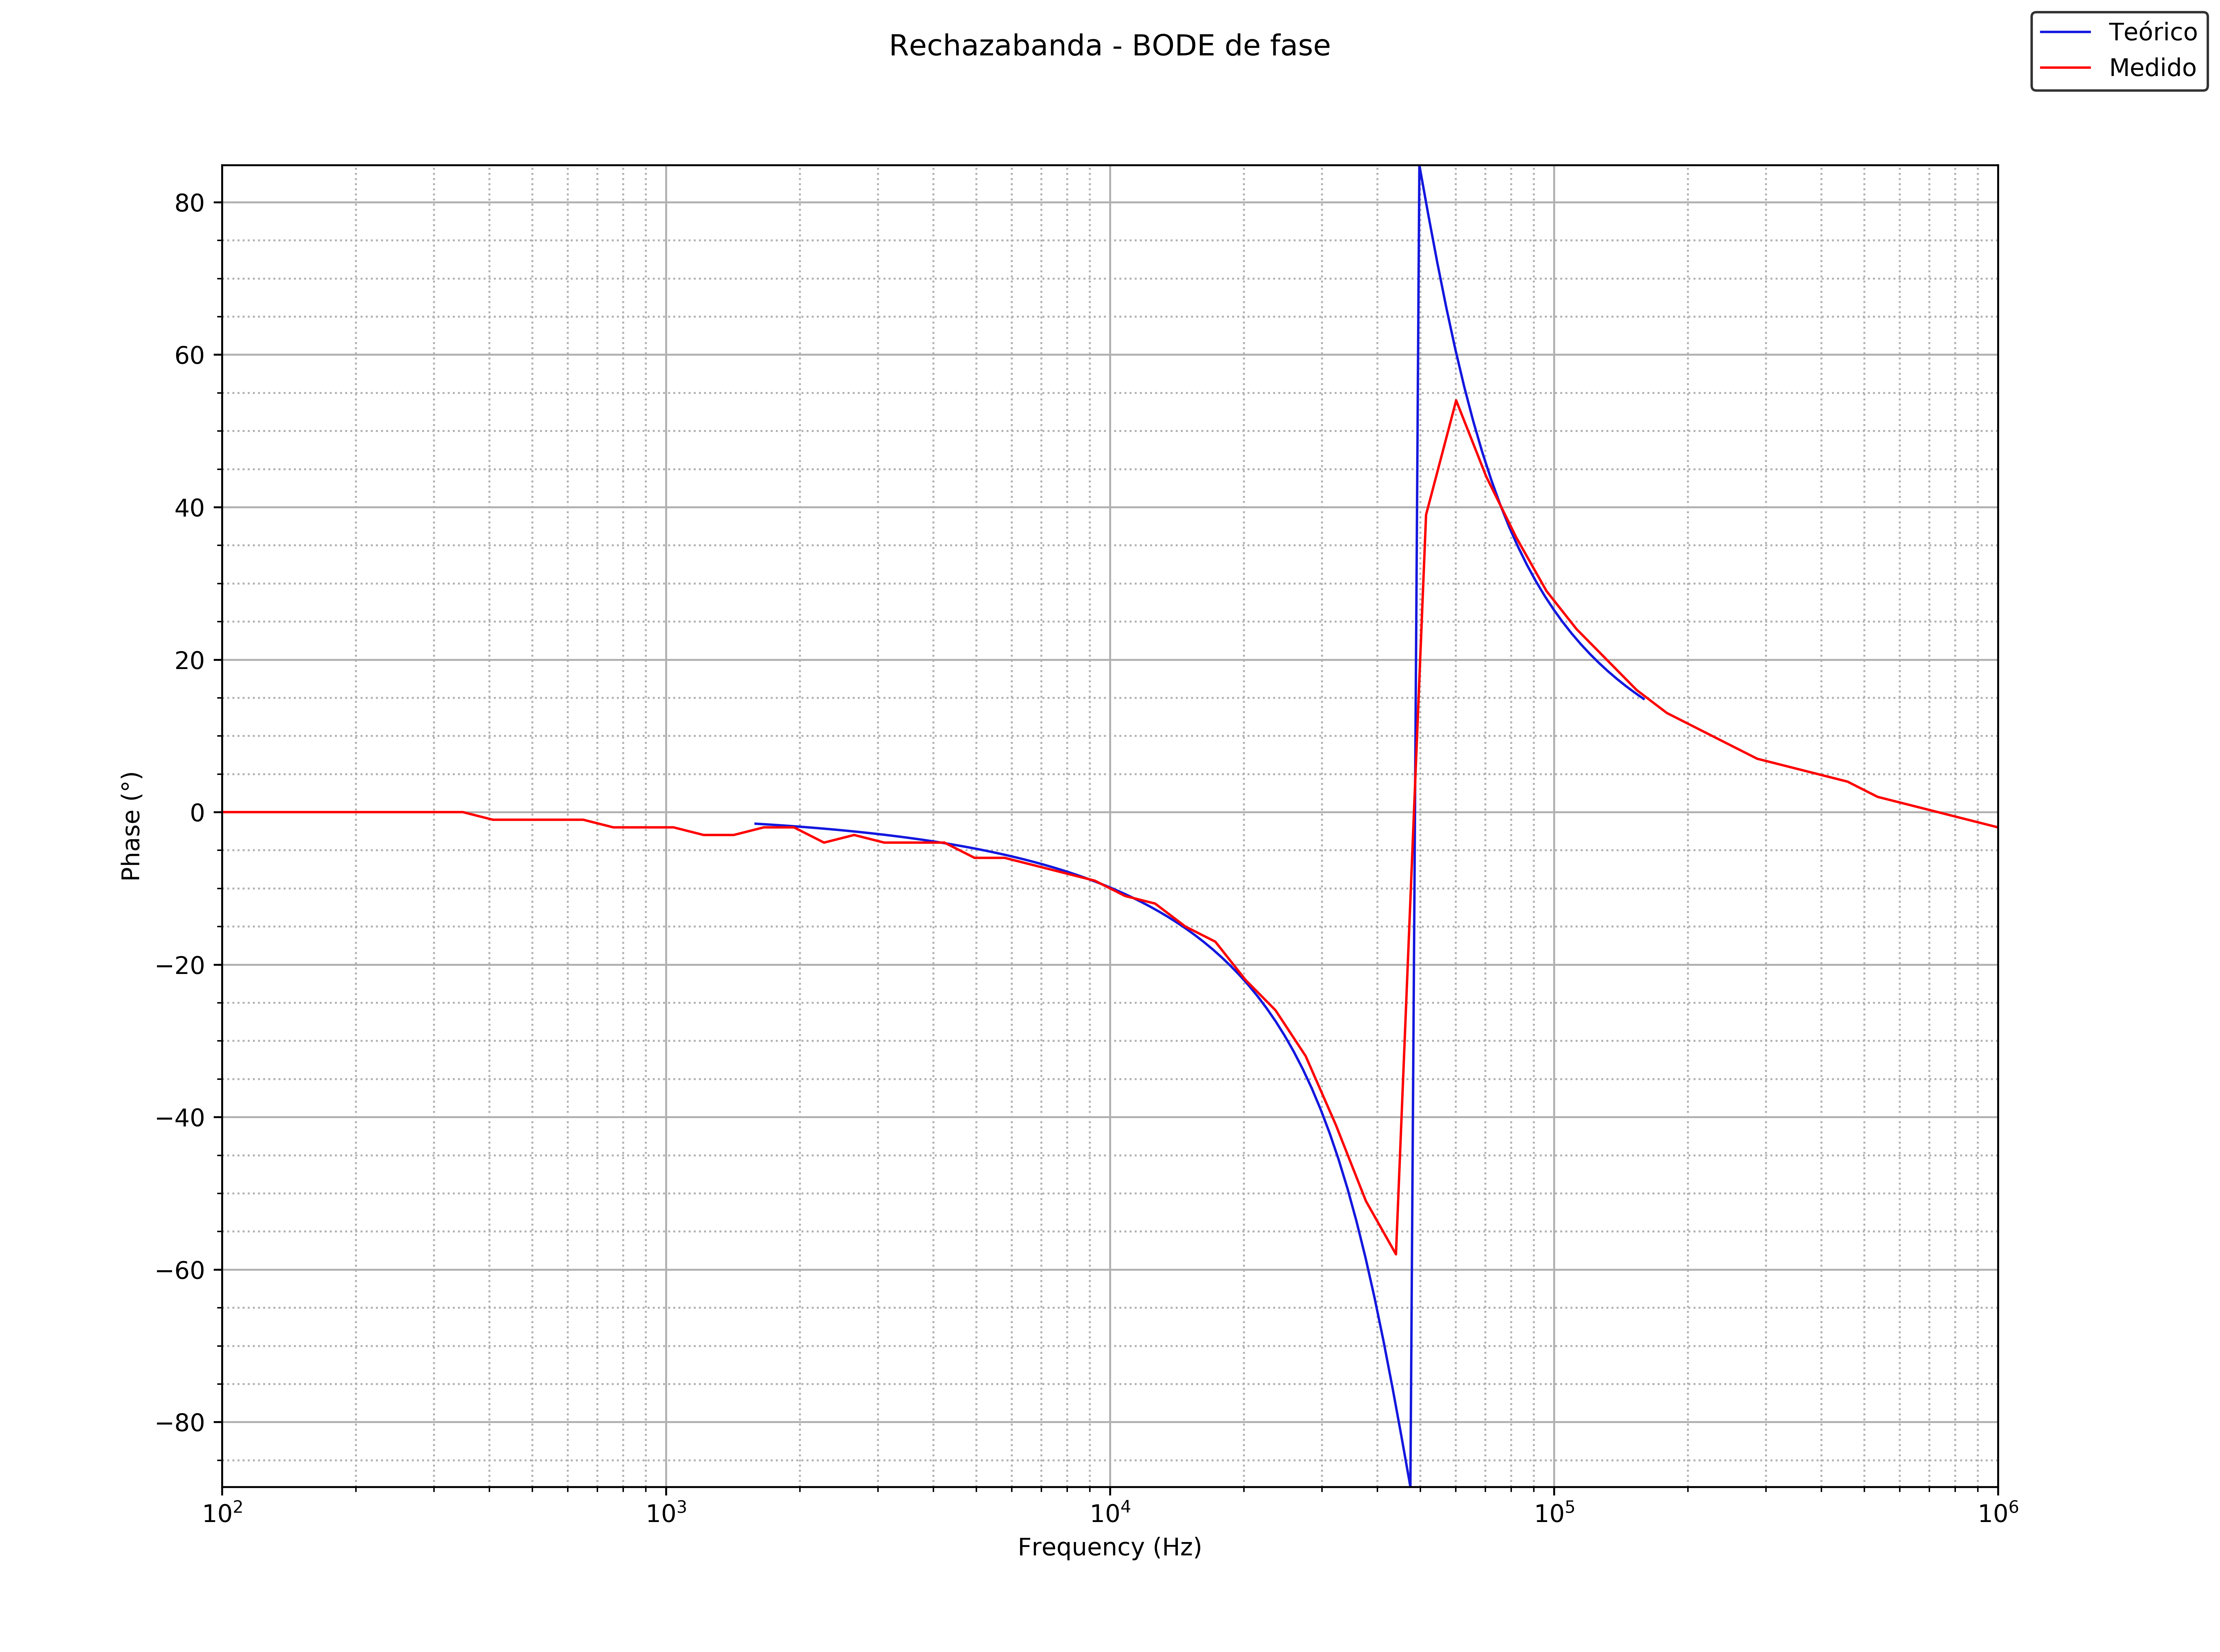
\includegraphics[scale=0.3]{./Recursos/ej4/rechazabanda_fase.png}
	\caption{Diagrama BODE de fase - Circuito rechazabanda}
\end{figure}

En ambos gr\'aficos se pueden observar diferencias en los datos recolectados respecto al comportamiento predicho del circuito. En l\'ineas generales, el pico de atenuaci\'on se produce en frecuencias similares. Se advierte que en la pr\'actica el nivel de atenuaci\'on en este pico es mucho menor que en el modelo te\'orico. Esto es porque el circuito no es de caracter ideal, y presenta variaciones en los par\'ametros caracter\'isticos que lo definen (inductancia, resistencia y capacitancia de sus componentes). Asimismo, se observa el mismo efecto en el caso de la fase. 
